% arara: lualatex: { shell: yes, interaction: nonstopmode, synctex: yes}
% arara: lualatex: { shell: yes, interaction: nonstopmode, synctex: yes}
% sarara: lualatex: { shell: yes, action: nonstopmode, synctex: yes}
% ssarara: lualatex: { shell: yes, action: nonstopmode, synctex: yes}
% asarara: lualatex: { shell: yes, action: nonstopmode, synctex: yes,  options: "-output-directory=_build"}
% asarara: lualatex: { shell: yes, action: nonstopmode, synctex: yes,  options: "-output-directory=_build"}
\documentclass{article}
\usepackage[ngerman]{babel}
\usepackage[no-math]{fontspec}

% \directlua{os.execute("cp basic/UbuntuL.ttf UbuntuL.ttf")}
% \directlua{os.execute("cp basic/UbuntuL.ttf UbuntuL.ttf")}
% \directlua{os.execute("c  p basic/UbuntuL.ttf UbuntuL.ttf")}

\usepackage{mwe}
\usepackage{luacode}
\usepackage{shellesc}
% \documentclassw[11pt, a4paper,ngerman]{article}
\usepackage{../latexBasic/basicff}


\usetikzlibrary{patterns} % preamble
\tcbuselibrary{skins} % preamble

\usepackage{tikz}
% \usepackage{PTSansNarrow}
\usetikzlibrary{matrix}

\usepackage{pgfplots}
\pgfplotsset{
 compat=newest
  }
\tcbset{colframe=red!75!black}
\newenvironment{proggen}{\begin{center}}{\end{center}}

\usepackage{array}
% \setmainfont[Path=/Applications/Microsoft Word.app/Contents/Resources/Fonts/]{Calibri.ttf}
% \setsansfont[Path=/Applications/Microsoft Word.app/Contents/Resources/Fonts/]{Calibri.ttf}
% \setmonofont[Path=/Applications/Microsoft Word.app/Contents/Resources/Fonts/]{Calibri.ttf}


\setmainfont[Numbers=OldStyle, Path=../latexBasic/]{UbuntuL.ttf}
\setsansfont[BoldFont = Ubuntu-B ,Numbers=OldStyle, Path=../latexBasic/]{UbuntuR.ttf}
\setmonofont[Numbers=OldStyle, Path=../latexBasic/]{UbuntuMonoR.ttf}
% \liningnums{\textbf{}}
% \oldstylenums{\textbf{}}


\newcolumntype{C}[1]{>{\centering\arraybackslash}m{#1}}

\oddsidemargin-10mm
\title{
\color{white}
 $\bullet$ \\ $\bullet$ \\ $\bullet$ \\
 \color{black}
 % \color{white}
 % $\bullet$ \\
 \color{black}
 \begin{center}
   Bachelor Project \\
   \color{white}
   $\bullet$ \\
   \color{black}
   Formula Mundi
 \end{center}
\color{white}
$\bullet$ \\
\color{black}
 \begin{center}
 % \includegraphics[scale=0.5]{./pictures/CaptainWarschburger.jpg}
\end{center}
 % \includegraphics{./pictures/wohnzimmer.png}
}
% \includegraphics{./pictures/asrock.png} Q1900M \\ \color{white} $\bullet$ \\ $\bullet$ \\ $\bullet$ \\ \color{black} \\ \apple \\ 10.10.3

\author{Daniel Krah}
% \date{1.6.2015}

\begin{document}
% \AddToShipoutPicture{\BackgroundPic}
\maketitle%
\newpage%
 \tableofcontents%
\newpage
%==================================================================================

% \newpage
% \sect{Überblick}
% \section{Überblick}

\sect{Was ist Formula Mundi}
Das Formula Mundi Filmfest ist ein unabhängiges und international ausgeschriebenes Nonprofit-Themenfestival, das 2003 an der Fachhochschule Schwäbisch Hall gegründet wurde. Während das Festival keinen festen Veranstaltungsort, keine festen Kooperationspartner sowie unregelmäßige Veranstaltungstermine hat, gibt es eimmer einen akademischen Kontext.\\

Die bisherigen Themen waren:
\begin{itemize}
  \item Die Weltformel
  \item Konsum und Kulturlandschaft
  \item Reflect Evolve Create
  \item concepts, struggles and changes within social structures
\end{itemize}

und wurden in den Veranstalltungsorten ausgerichtet.
\begin{itemize}
  \item Schwäbisch Hall
  \item Kairo
  \item Tallinn
\end{itemize}

Das kommende Festival wird in Fulda mit dem Thema \glqq{}Impact on tomorrow\grqq{} stattfinden und folgende Kategorien sind gesucht:

\begin{itemize}
  \item Dokumentation
  \item Animation oder Experimentell
  \item Erzählung (Kurz oder Langfilm)
\end{itemize}

\sect{Formula Mundi Online}

Das Ziel dieses Projektes ist die Ausarbeitung einer Strategie wie man das Filmfestival Online abhalten könnte.
Grund hierfür sind die noch anhaltenden Auflagen für Veranstaltungen durch Corona.\\

Dabei gehe ich auf die Punkte ein: \\

\begin{itemize}
  \item Video-Plattformen
  \item Unterschiedliche Arten der Videoveröffentlichung.
  \item Interaktionsmöglichkeiten
\end{itemize}

\newpage
\sect{Videoplattformen und ihre Veröffentlichungsvarianten}

\sub{Bereitstellungsvarianten}
Grundsätzlich gibt es 4 verschiedene Möglichkeiten der Filmbereitstellung: \\

\begin{itemize}
  \item Selbst gehostete Filme auf eigener Webseite.
  \item Fertig produzierter Film auf Videoplattform
  \item Livestream auf Videoplattform
  \item Youtube Premiere
\end{itemize}
{\vspace{-0.7cm}}

\subsub{Selbst gehostete Filme auf eigener Webseite}
Hierbei werden die eingereichten Filme auf der eigenen Webpräzens gezeigt.\\
Die Filmdateien können hierbei auf dem eigenen Server liegen oder über einen CDN zur Verfügung gestellt werden. \\
Content Delivery Networks haben hierbei den Vorteil das die Netzwerkauslastung des eigenen Webseiten-Servers gering bleibt. \\

Bekannte CDN's sind Akamai, Microsoft Azure, Amazon Web Services (AWS) sowie Cloudflare.

\subsub{Fertig produzierter Film auf Videoplattform}

Beim fertig produzierten Video auf einer Videoplattform ist es ähnlich wie beim hosten auf einem CDN. Der eigene Server wird entlastet aber zusätzlich stehen dem Nutzer häufig unteschiedliche Videoauflösungen zur Verfügung. Das ist ein großer Vorteil für Zuschauer welche über ein Mobiltelefon zuschauen möchten. Dort sind sie höheren Auflösungen oft nicht nötig und falls der Zuschauer über seinen Mobilfunkvertrag schaut wird sein Datenvolumen geschont. \\
Ein Nachteil können aber die AGB's des Anbieters sein und es kann vorkommen das Videos fälschlicherweise gesperrt werden.

\subsub{Livestream auf Videoplattform}
Im Unterschied zum fertig produzierten Video kann das Video zumindest während des erstmaligen Vorführen nicht geblockt werden.
Danach gibt es für den Verbleib des Videos verschiedene Möglichkeiten. \\
Bei manchen Plattformen ist das Video nur während des Livestreams zu sehen, bei anderen Plattformen ist das gestreamte Video auch danach noch ansehbar.\\

Beim Livestream müssen die Daten in Echtzeit zum Server übertragen werden.
Die maximale Bildqualität hängt daher stark von dem zur Verfügung stehenden Internetanschluss ab.
Während des Livestreams ist es möglich einen Livechat zur nutzen.
Auch wenn die Datenrate durch den Upload begrenzt ist hat man die Möglichkeiten einen Film in eine Anmoderierung sowie nachfolgende Diskussionsrunde einzubinden.




\subsub{Youtube Premiere}
Eine Youtube Premiere ist ein Mix aus vorproduziertes Video und Livestream.
Das vorproduzierte Video kann zum Zeitpunkt der Veröffentlichung nicht vorgespult werden.
Es ist möglich einen Livechat zu aktivieren um während der Vorführung zu kommunizieren.




\newpage
\sub{Aktuelle Videoportale (Land, Erscheinungsjahr)}

Viele bekannte Portale wie Clipfish (DE), MyVideo (DE), Sevenload(DE), Vevo (USA) gibt es nicht mehr.\\
Vevo vertreibt seine Videos nun über Youtube.\\


\begin{itemize}
  \item Europa
  \begin{itemize}
    \item alugha(DE 2014) kostenpflichtig und es sind nur 180 Minuten frei.
    \item item Dailymotion (FR 2005) Kein Livestreaming und die Videoübersicht ist recht unübersichtlich gestaltet.
  \end{itemize}
  \item Noch in Europa
  \begin{itemize}
    \item LiveLeak (GB 2006) verlinkt nur noch auf Youtubevideos
  \end{itemize}
  \item Amerika
  \begin{itemize}
    \item Twitch (USA 2011 Amazon) Streaming für Spieler,
    \item Vimeo (USA 2004) kostenpflichtig Livestreams erst ab 70€ im Monat,
    \item Youtube (USA 2005 Alphabet)
  \end{itemize}
  \item Asien
  \begin{itemize}
    \item Youku (China 2006) Nur in chinesischer Sprache
    \item TikTok (China 2016) Nur Miniclips
  \end{itemize}
\end{itemize}


{\vspace{0,2cm}}
\textbf{Fazit:}
Bleibt prinzipiell nur Youtube ...

\sub{Fazit: Youtube}

Youtube ist eine Videoplattform welche von Youtube LLC betrieben wird. \\
Youtube LLC eine Tochtergesellschaft von Google LLC, die wiederum eine Tochtergesellschaft von Alphabet Inc. ist.

\begin{flushright}
  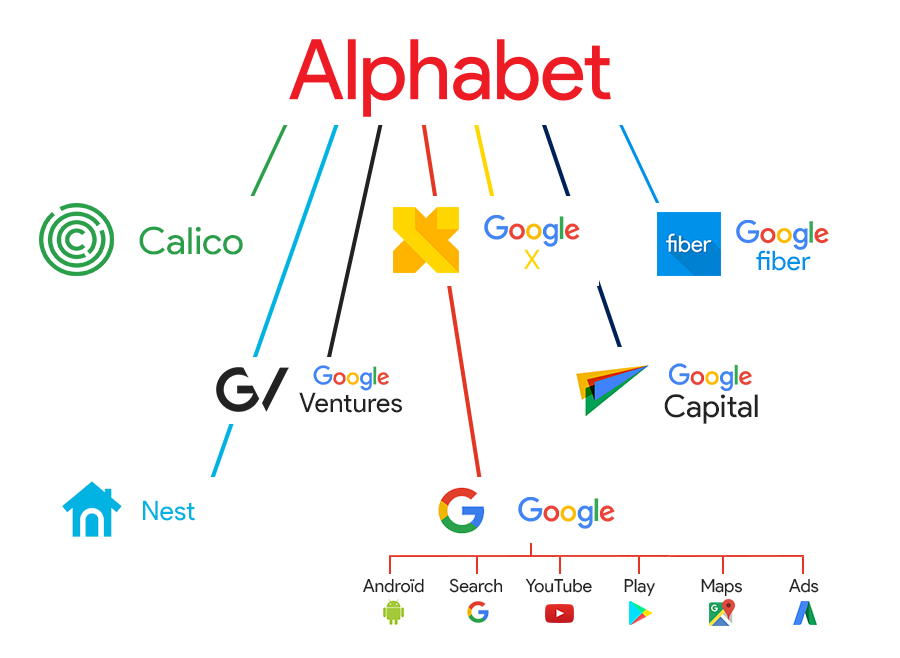
\includegraphics[scale=1.3]{./pictures/alphabet.png}
\end{flushright}

{\vspace{-2,5cm}}
Funktionen die Youtube bietet:
\begin{itemize}
  \item live-Streaming (mit Live-Chat)
  \item Produzierte Videos
  \item Video Premieren \\ (Vorproduzierte Videos. verhalten sich wie Livestream (mit Live-Chat, können nicht vorgespult werden bei der Premiere.))
\end{itemize}
\newpage

Neben der werbefreien Veröffentlichung können Videos auch Monetarisiert werden. Dies geschieht bei Youtube über den Google Dienst AdSense, welcher oft auch auf normalen Webseiten benutzt wird. \\
Hauptberufliche Youtuber nutzen diesen Dienst zwar auch, aber zum  \quote{Davon Leben} reicht dies in der Regel nicht.\\
Oftmals reichen die Einahmen hiervon gerade so um die Produktionskosten des Videos wieder rein zu holen. \\
Die meisten Youtuber finanzieren diese sich über Affiliate-Marketing-Links was einer Vermittlungsprovision entspricht. Hierbei werden Produktreviews gemacht und dann Links zu verschiedenen Shops in die Videobeschreibung gepackt über die der Youtuber dann ein paar Euro bekommt wenn der Zuschauer über diesen das Produkt kauft. \\
Ebenso ist es mittlerweile üblich das Firmen direkt Youtuber sponsern und im Gegenzug dann eine 1-3 minütige Produktvorstellung ins Video eingebunden bekommen.\\
Der Vorteil hierbei ist für beide Seiten das Google als \quote{Zwischenhändler} (Welche ja auch eine Provision möchte) wegfällt. \\
Dadurch bekommt der Youtuber in der Regel höhere Einnahmen als über Youtube. Die Firma kann hierdurch gezielter werben und ist nicht auf den Google-Algorithmus angewiesen.\\

Aber es gibt auch Youtube Netzwerke wie \quote{Funk} des öffentlich rechtlichen Rundfunks welche Youtuber sponsern.\\

Nennenswerte Beispiele sind hierbei:
\begin{itemize}
  \item maiLab von Mai Thi Nguyen-Kim produziert vom SWR
  \item Browser Ballett von Christian Brandes (und vielen weiteren) produziert von Steinberger Silberstein GmbH
  \item MrWissen2go von Mirko Drotschmann produziert von MDR und SWR
  \item STRG F ist ein wöchentliches Doku-Format welches vom NDR produziert wird
\end{itemize}


Funk finanziert aber auch viele Serien. Mit \quote{Wach} im Jahre 2018 wurde erstmalig ein Film finanziert

\newpage
\sub{Verschiedene Youtube-Streaming-Setups}
\begin{table}[h]
  \begin{adjustwidth}{-1cm}{-1cm}% adjust the L and R margins by 1 inch
    \begin{center}
      \textbf{Verschiedene Youtube Streaming Setups}
      \begin{tabular}{|p{3cm}|p{3cm}|p{3cm}|p{3cm}|p{3cm}|p{3cm}|}
        \hline
                          &  Geeignet für                                                         & Programmgestaltungsformat & Komplexität der Einrichtung & Erforderliche Mindestausrüstung & Anwendungsfall \\ \hline
        Mobilgerät        & Streaming unterwegs                                                   & Schnell und einfach       & Gering                      & Mobiltelefon mit Kamera & Livestream in wenigen Schritten über ein Handy startet \\ \hline
        Webcam            & Einfache Webcam-Streams                                               & Schnell und einfach       & Gering                      & Computer mit Webcam & Livestream mit wenigen Klicks starten\\ \hline
        Jetzt Streamen    & Reproduzierbare Livestreams, die eine einmalige Einrichtung erfordern & Produziert                & Mittel/Hoch                 & Computer mit Webcam und Streamingsoftware & Eine Liveadresse für wiederholbare Livestreams \\ \hline
        Veranstaltungen   & Livestream-Einrichtung mit vielen Anpassungsmöglichkeiten             & Tent-Poling-Video         & Hoch                        & Computer, Kamera, Streamingsoftware  & Eine benutzerdefinierte Live-Veranstaltung erstellen, welche auch ein Multicamstream sein kann. \\ \hline
        Youtube Premiere  & Produziertes Video mit Livechat                                       & Tent-Poling-Video         & Mittel/Hoch                 & Computer, Streamingsoftware & Ein einmalig nicht vorspulbares vorproduziertes Video welches Interaktionsmöglichkeiten bietet \\ \hline
      \end{tabular}
    \end{center}
  \end{adjustwidth}
\end{table}

















% \begin{table}[ht]
%   \begin{tabular}{|p{3cm}|p{3cm}|p{3cm}|p{3cm}|p{3cm}|}
%     \hline
%     &  Mobilgerät         & Webcam & Jetzt Streamen & Veranstalltungen \\ \hline
%     Geeignet für                    & Streaming unterwegs & Einfache Webcam-Streams & Reproduzierbare Livestreams, die eine einmalige Einrichtung erfordern & Livestream-Einrichtung mit vielen Anpassungsmöglichkeiten \\ \hline
%     Programmgestaltungsformat       & Schnell und einfach & Schnell und einfach & Produziert & Tent-Poling-Video \\ \hline
%     Komplexität der Einrichtung     & Gering & Gering & Mittel/Hoch & Hoch \\ \hline
%     Erforderliche Mindestausrüstung & Mobiltelefon mit Kamera & Computer mit Webcam & Computer mit Webcam und Streamingsoftware & Computer Kamera Streamingsoftware \\ \hline
%     Anwendungsfall                  & Livestream in wenigen Schritten über ein Handy starteb & Livestream mit wenigen Klicks starten & Eine Liveadresse für wiederholbare Livestreams & Eine benutzerdefinierte Live-veranstaltung erstellen, welche auch ein Multicamstream sein kann. \\ \hline
%   \end{tabular}
% \end{table}

% \begin{center}
% {\vspace{-15cm}}

% \clearpage
\sect{Streaming Voraussetzungen}
\sub{Internetverbindung}

\subsub{Übersicht}
In Deutschland hat sich der Markt der Internetanbieter recht bereinigt.
Bei Kabelanschlüssen gibt es durch Fusionen nur noch die Anbieter Vodafone und PŸUR.
Wobei Vodafone nun mit weiten Abstand der Größte Anbieter ist. \\
Bei den DSL Anbietern gibt es beispielsweise Telekom, Vodafone, 1\&1, O$^2$. \\
Von den Kosten her schneidet die Telekom am besten ab. \\
Nachfolgend kommen die aktuellen Tarife von der Telekom (DSL) sowie Vodafone (Kabel).
Tarife spiegeln aber nur grob das wieder was man maximal erwarten kann.
Ein Blick in die Leistungsbeschreibungen zeigt einem was man realistisch erwarten kann.\\
Auch sollte einem klar sein das bei einem 1000Mbit Tarif diese technisch nicht voll nutzbar sind.
Da es bei Netzwerkkommunikation immer Protokolldaten und Nutzdaten gibt können niemals 1000 Gigabit an Nutzdaten übertragen werden.\\

In einem Heimnetzwerk können beispielsweise nur \textasciitilde 923 Mbit (Gigabit-Netzwerk)/ \textasciitilde 92,3 Mbit (100 Megabit-Netzwerk) übertragen werden.
Bei einer Übertragung über das Internet ist der Anteil der Protokolldaten noch höher.
Der zu erwartenden Wert sieht man unter \quote{Normalerweise zur Verfügung stehend}.
Die Unterschiede zwischen VDSL-Technologie und Fiber-Technologie ergeben sich dadurch das bei der Fiber-Technologie weniger Fehlerkorrektur notwendig ist.\\

% \newpage
\subsub{Aktuelle Tarife}

{\vspace{-0.6cm}}
\begin{center}
  \textbf{Telekom} \\
  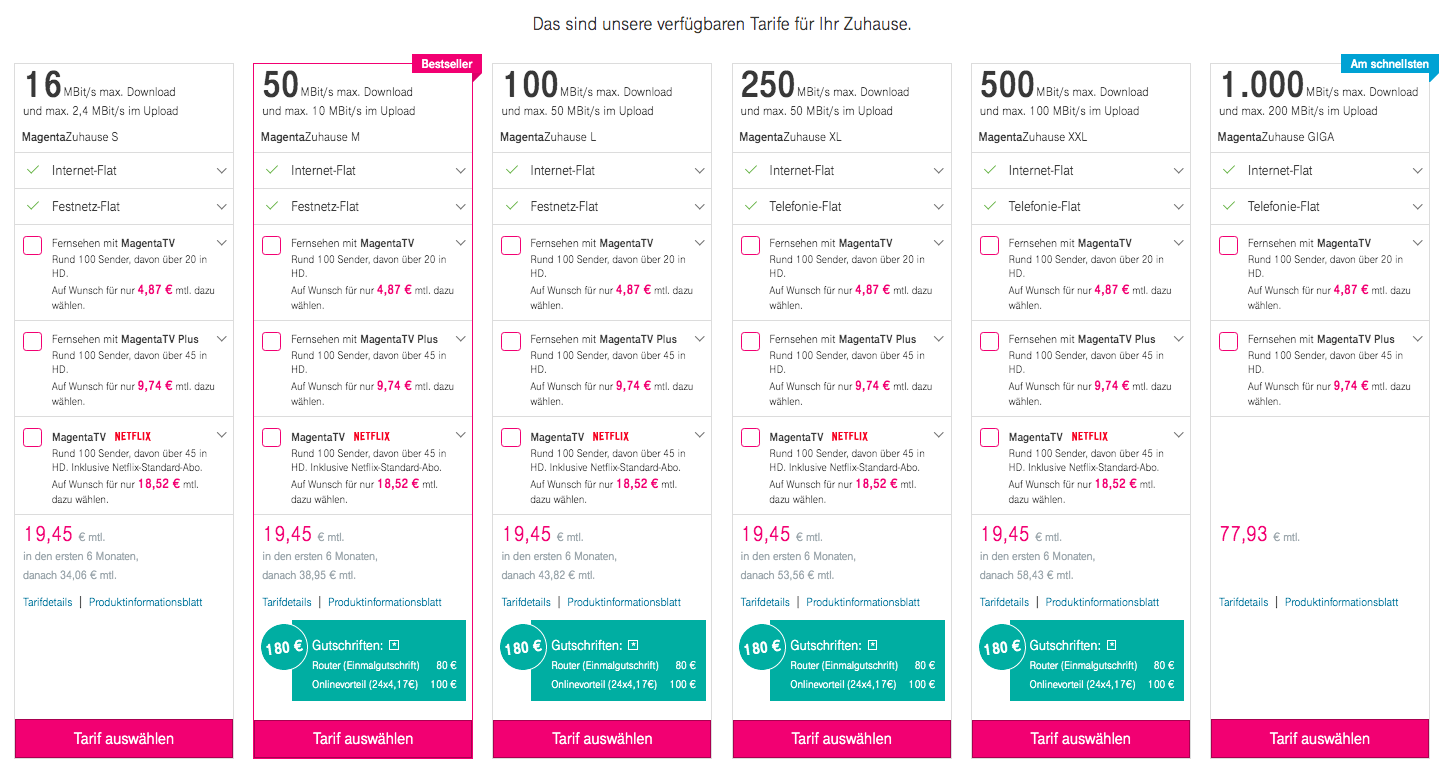
\includegraphics[scale=0.35]{./pictures/t-dsl.png}
\end{center}

{\vspace{-0.7cm}}
\begin{center}
  \textbf{Vodafone Tarif-Übersicht} \\
  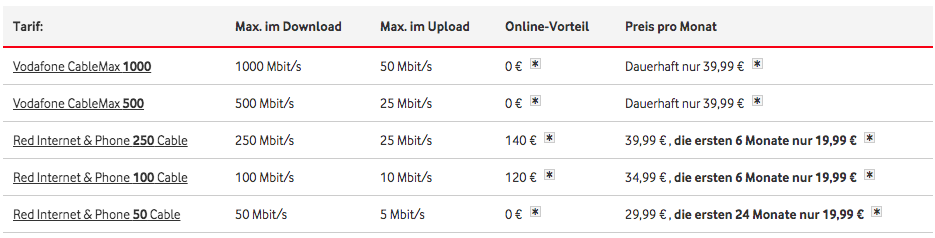
\includegraphics[scale=0.54]{./pictures/vodafoneKabel.png}
\end{center}

Die Telekom hat bei den Tarifen 250, 500, 1000 kürzlich den Upload reduziert, aber den Preis teils deutlich gesenkt.\\




  {\vspace{-0.4cm}}
  \begin{table}[ht]
    \begin{center}
    % \caption{alte Telekom Tarife}
    \label{alte Telekom Tarife}
    \begin{tabular}{|>{\raggedleft}p{3.5cm}| >{\centering}p{1cm}| >{\centering}p{1cm}| >{\centering}p{1cm}|}
      \hline
      \multicolumn{4}{|c|}{Frühere Datenraten} \tabularnewline \hline
      Download in Mbit/s & 250 & 500 & 1000 \tabularnewline
      \hline
      Upload in Mbit/s & 100 & 200 & 400 \tabularnewline \hline
    \end{tabular}
    \end{center}
  \end{table}

% \clearpage

\newpage

% \begin{minipage}


\begin{table}[ht]
  {\vspace{-1.5cm}}
  \begin{center}
    \textbf{Leistungsbeschreibungen der verschiedenen Tarife.}
  \end{center}
  \begin{center}
  % \caption{alte Telekom Tarife}
  \label{alte Telekom Tarife}
  \begin{tabular}{>{\centering}p{0.5\textwidth} >{\centering}p{0.5\textwidth}}
        \textbf{DSL 16} \\ 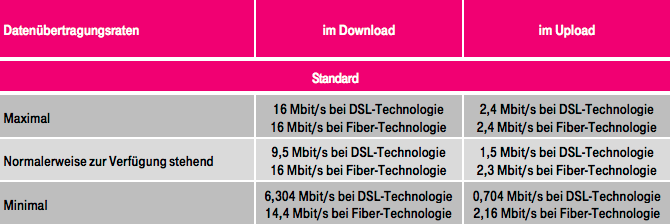
\includegraphics[width=0.5\textwidth, height=3cm]{./pictures/dsl16vertrag.png} & \textbf{DSL 50} \\ 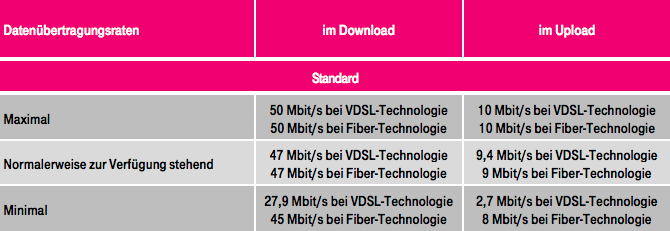
\includegraphics[width=0.5\textwidth, height=3cm]{./pictures/dsl50vertrag.png} \tabularnewline
        \textbf{DSL 100} \\ 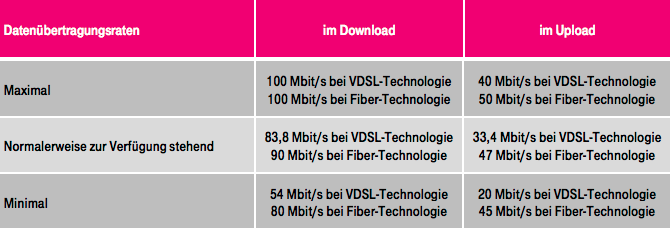
\includegraphics[width=0.5\textwidth, height=3cm]{./pictures/dsl100vertrag.png} & \textbf{DSL 250} \\ 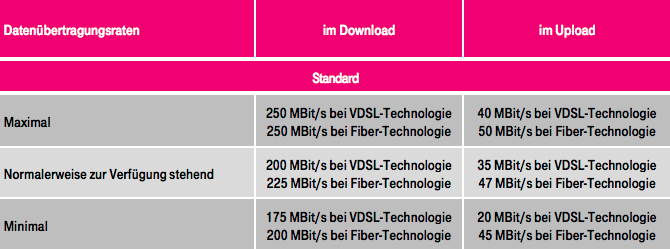
\includegraphics[width=0.5\textwidth, height=3cm]{./pictures/dsl250vertrag.png} \tabularnewline
        \textbf{DSL 500} \\ 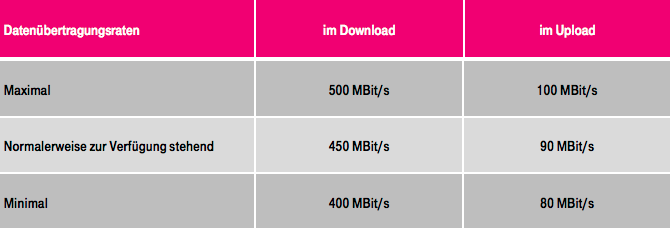
\includegraphics[width=0.5\textwidth, height=3cm]{./pictures/dsl500vertrag.png} & \textbf{DSL 1000} \\ 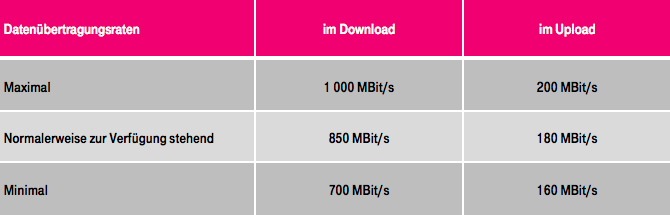
\includegraphics[width=0.5\textwidth, height=3cm]{./pictures/dsl1000vertrag.png} \tabularnewline
        &  \tabularnewline
        &  \tabularnewline
        \textbf{cable 50} \\ 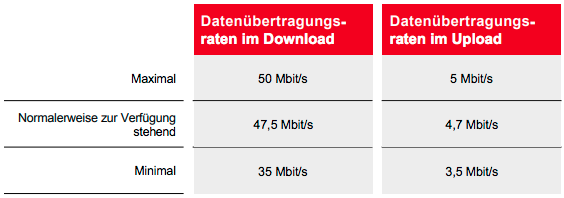
\includegraphics[width=0.5\textwidth, height=3cm]{./pictures/voda50.png} & \textbf{cable 100} \\ 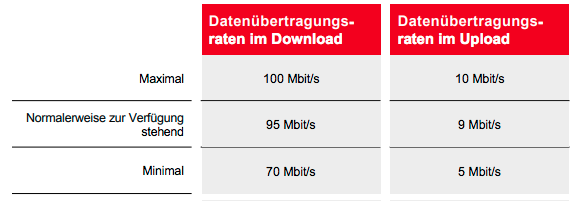
\includegraphics[width=0.5\textwidth, height=3cm]{./pictures/voda100.png} \tabularnewline
        \textbf{cable 250} \\ 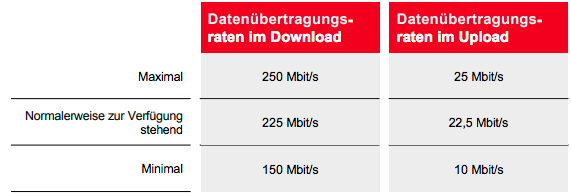
\includegraphics[width=0.5\textwidth, height=3cm]{./pictures/voda250.png} & \textbf{cable 500} \\ 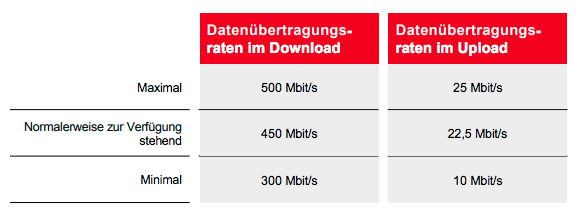
\includegraphics[width=0.5\textwidth, height=3cm]{./pictures/voda500.png} \tabularnewline
        \textbf{cable 1000} \\ 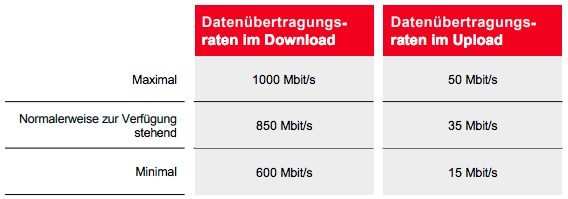
\includegraphics[width=0.5\textwidth, height=3cm]{./pictures/voda1000.png} &  \tabularnewline
  \end{tabular}
  \end{center}
\end{table}
\clearpage

% \begin{table}[ht]
%   {\vspace{-2cm}}
%   \begin{center}
%   % \caption{alte Telekom Tarife}
%   \label{alte Telekom Tarife}
%   \begin{tabular}{>{\centering}p{0.5\textwidth} >{\centering}p{0.5\textwidth}}
%         \textbf{DSL 16} 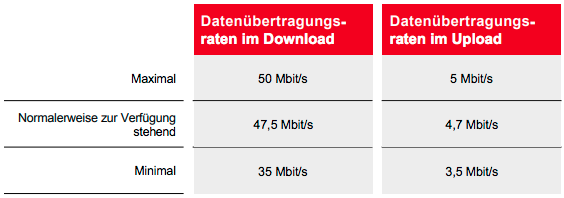
\includegraphics[width=0.4\textwidth, height=2.4cm]{./pictures/voda50.png} & \textbf{DSL 50} 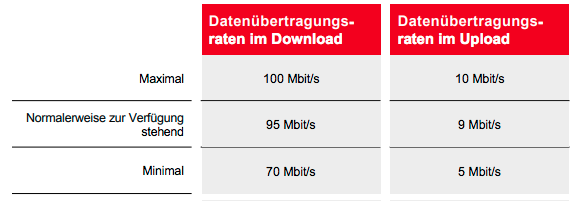
\includegraphics[width=0.4\textwidth, height=2.4cm]{./pictures/voda100.png} \tabularnewline
%         \textbf{DSL 100} 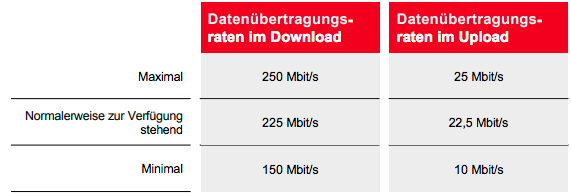
\includegraphics[width=0.4\textwidth, height=2.4cm]{./pictures/voda250.png} & \textbf{DSL 250} 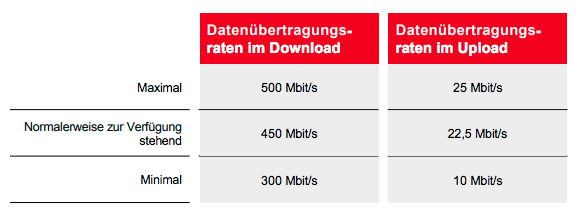
\includegraphics[width=0.4\textwidth, height=2.4cm]{./pictures/voda500.png} \tabularnewline
%         \textbf{DSL 500} 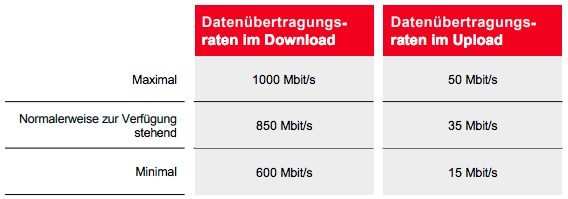
\includegraphics[width=0.4\textwidth, height=2.4cm]{./pictures/voda1000.png} &  \tabularnewline
%   \end{tabular}
%   \end{center}
% \end{table}
% \end{minipage}
% {\vspace{-0.7cm}}
% \begin{center}
%   \textbf{Vodafone Tarif-Übersicht} \\
%   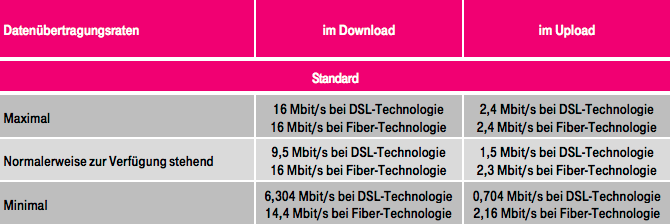
\includegraphics[scale=0.54]{./pictures/dsl16vertrag.png}
% \end{center}

\newpage
\subsub{Übersicht über die eigene Internetverbindung}

Zu Hause habe ich aktuell den kleinsten Telekom Vertrag, welcher aber mit 13€ für Internet + Telefon sehr günstig ist.
Von daher halten sich hier die Streaming-Möglichkeiten in Grenzen. \\
Da die Hochschule ans DFN angeschlossen ist und einen redundant synchronen 1 Gigabit Anschluss hat sind dort prinzipiell perfekte Streamingvoraussetzungen gegeben. Aber auch hier muss man beachten das diese nicht überall verfügbar sind. So übertragen die Wlan Router oft nur 600 Mbit/s im 2,4 GHz und 5 GHz Band und es ist ein geteiltes Medium, das heisst die Bandbreite steht einem nicht exclusiv zur Verfügung.

Relevant für Liveübertragungen ist hierbei der Upload welcher die maximal erreichbare Bildauflösung und Bildqualität beeinflusst.


\small
\color{black}
\vspace{0.3cm}
\begin{center}
  \begin{tikzpicture}
    \clip node (m) [matrix,matrix of nodes,
    fill=fulda_green!20,inner sep=0pt,
    nodes in empty cells,
    nodes={minimum height=1cm,minimum width=2.6cm,anchor=center,outer sep=0,font=\sffamily},
    row 1/.style={nodes={fill=fulda_green,text=white}},
    column 1/.style={nodes={fill=fulda_green,text=white,align=left,text width=3cm,text depth=0.5ex}},
    column 2/.style={text width=12cm,align=left,every even row/.style={nodes={fill=white}}},
    column 3/.style={text width=3cm,align=center,every even row/.style={nodes={fill=white}},},
    row 1 column 1/.style={nodes={fill=fulda_green}},%									1. spalte oben
    prefix after command={[rounded corners=4mm] (m.north east) rectangle (m.south west)}
    ] {
    & $\ \ $ T-DSL 16.0000 Fiber to the Curb\\
    $\ \ $ Download   	  & $\ \ $ 14,4 Mbit/s \\
    $\ \ $ Upload 				& $\ \ $ 2,16 Mbit/s \\
    };
  \end{tikzpicture}
\end{center}
\normalsize

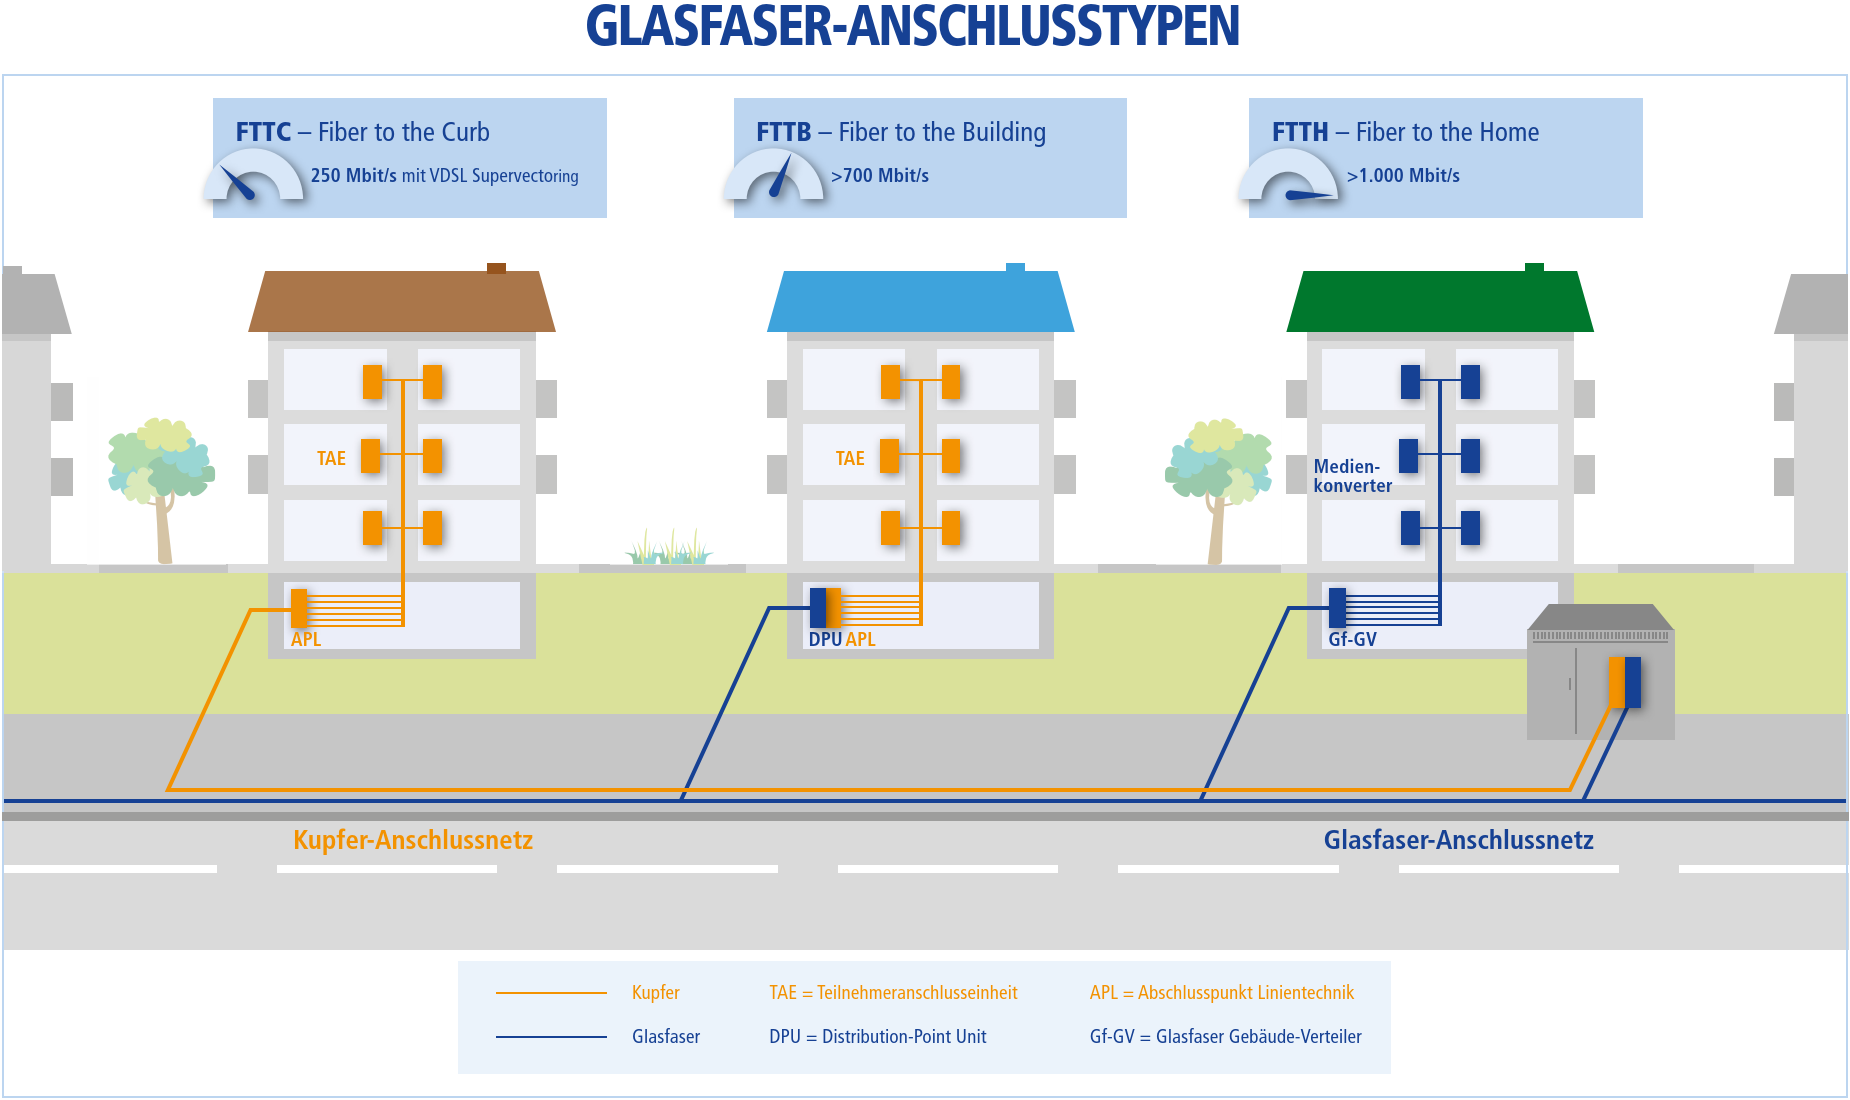
\includegraphics[width=\textwidth]{./pictures/fttc.png}

{\vspace{0.5cm}}

Der Internetanschluss wird über  \quote{Fiber to the curb} bereitgestellt. Hierfür wurden von der Rhön Energie Glasfaser-Leitungen bis in den Verteilerkasten gelegt. Die letzte Meile wird über Kupfer übertragen, welches seit ein paar Monaten nun auch mit VDSL2 geschieht. Dadurch sind nun Datenraten bis 250Mbit im Download verfügbar. Aber weil die Telekom den Upload halbiert hat ist dieser Tarif aber grade fürs Streaming unintressanter geworden. \\

50 Mbit/s im Upload wären prinzipiell aber trotzdem für alle Streaming-Auflösungen und fast alle Datenraten ausreichend.



\subsub{Überprüfen des Heimnetzes}
% \subsub{Überprüfen der Internetverbindung}

Für das Überprüfen der Internetverbindung muss man erst mal alle Störungen im Heimnetz ausgeschlossen haben. Der einfachste Weg ist ein direkt verbundenes fertig konfektioniertes Netzwerkkabel zwischen dem PC und dem Internetrouter. Da die Netzwerkkarte am Hackintosh (Eigenbau PC auf welchem MacOS läuft) wegen des schlechten Treiber recht instabil läuft verwende ich für alle Datenübertragungen Wlan.\\
Bei der Nutzung von Wlan ist darauf zu achten das ein möglichst nicht von einem anderen Wlan-Router genutzten Kanal verwendet wird. Wenn sich Wlan-Netzwerke überschneiden wie unten im Bild beim 2,4 GHz Band dann kann es zu Einbusen kommen wenn bei Router viele Daten übertragen. Das Wlan über die AVM Fritzbox wurde nur für dieses Foto aktiviert, da dieses bei der Fritzbox Wlan 7490 dermaßen schlecht ist, sodass es in der Regel nur sehr eingeschränkt nutzbar ist.
Da ich auf dem Land in einer Souterrain-Wohnung lebe, welche vor dem Fenster zusätzlich gut bepflanzt ist, werden die Wlan-Router der Nachbarn komplett abgeschirmt.\\


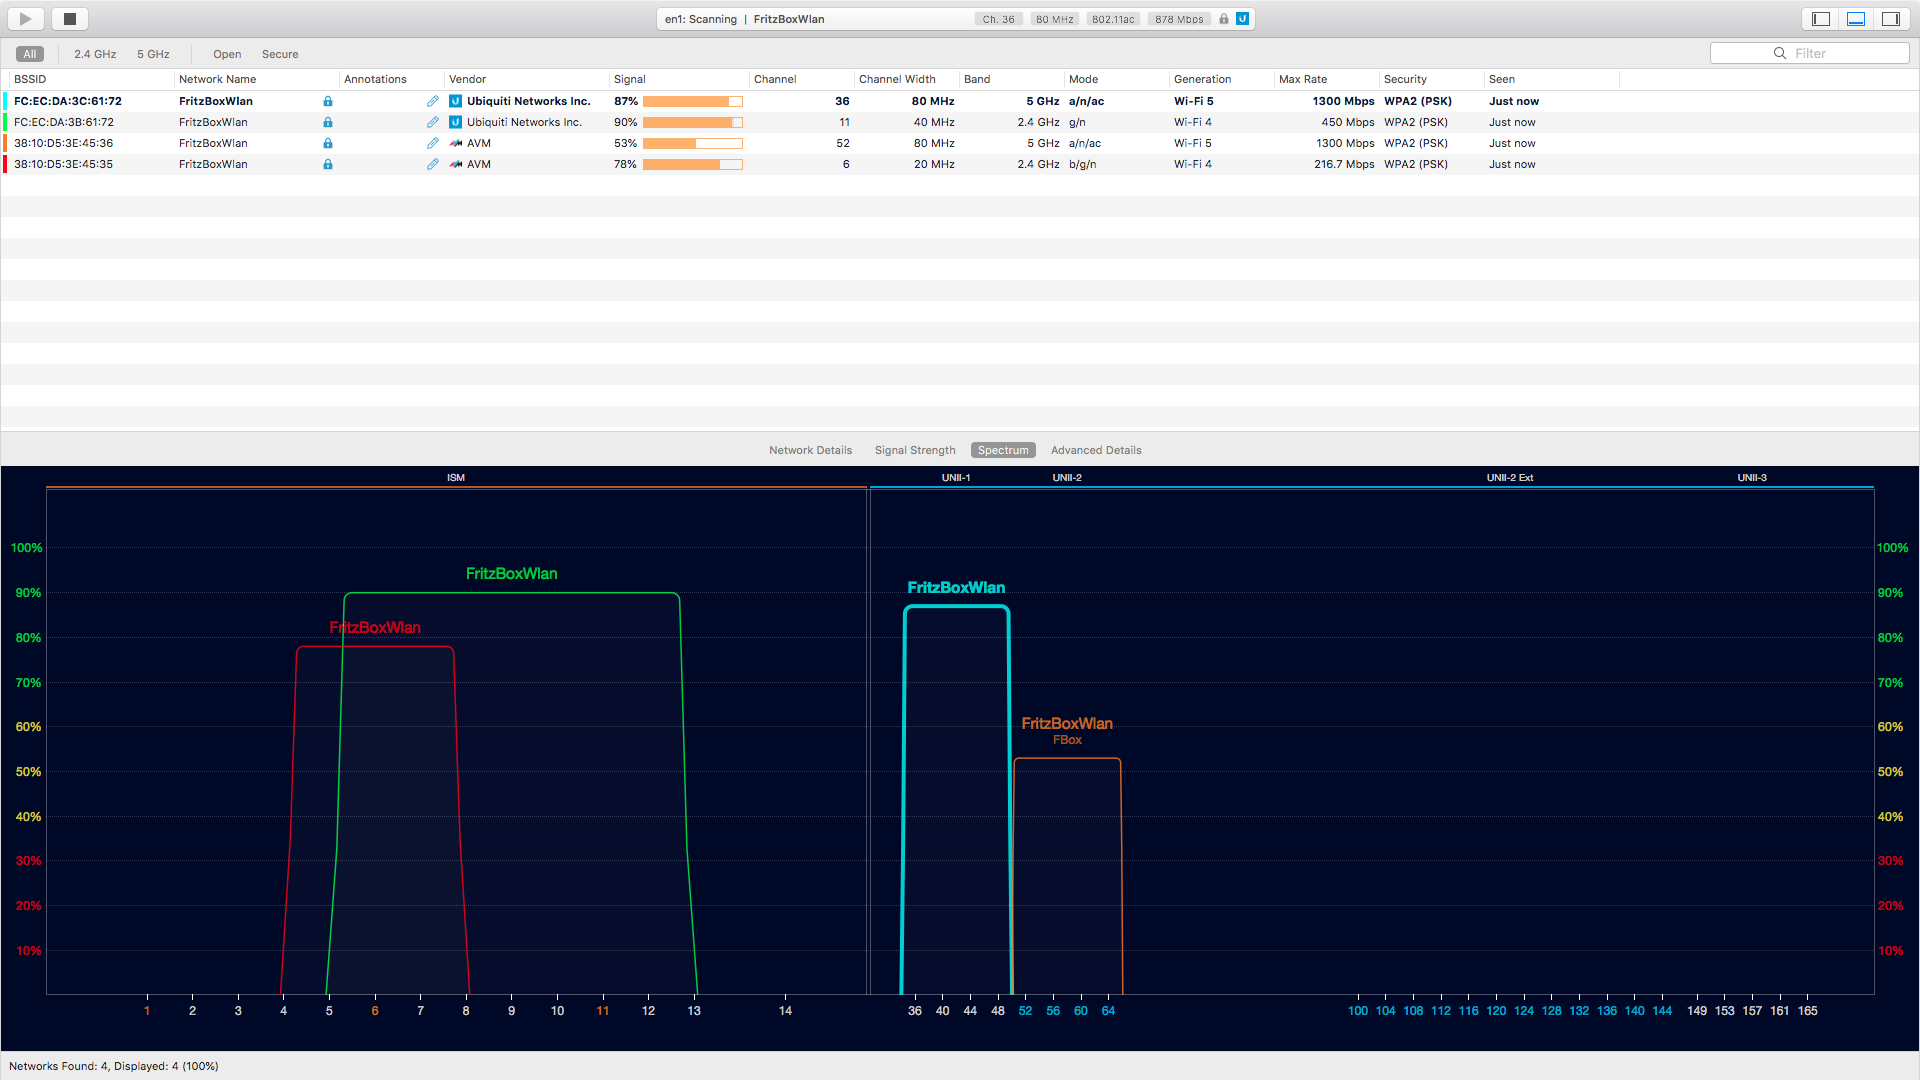
\includegraphics[width=\textwidth]{./pictures/wifiNetworks.png}

Des weiteren sollte man kontrollieren ob nicht irgendwo im Netzwerk irgendwelche Stromsparfunktionen aktiv sind.

{\vspace{0.2cm}}
\begin{center}
  % \textbf{DSL-Informationen der FritzBox} (ADSL 2+ = VDSL)\\
  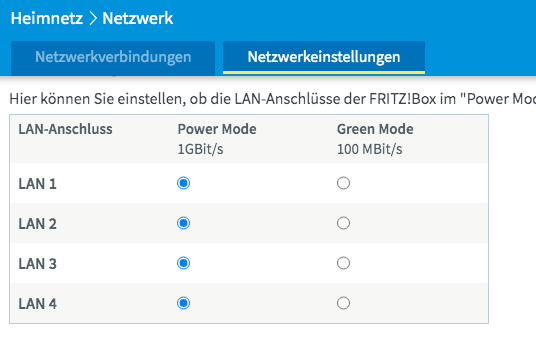
\includegraphics[scale=0.40]{./pictures/powerSaveNetwork.png}
\end{center}

Durch magnetische Felder und andere Störungen im Haus kann es aber vorkommen, \\
dass die Netzwerkgeräte die Gigabitverbindung nicht synchronisiert bekommen.
Dann fallen diese beispielsweise auf 100 Megibit oder im schlimmsten Fall auch auf 10 Megabit zurück.
% {\vspace{0.2cm}}
\begin{center}
  % \textbf{DSL-Informationen der FritzBox} (ADSL 2+ = VDSL)\\
  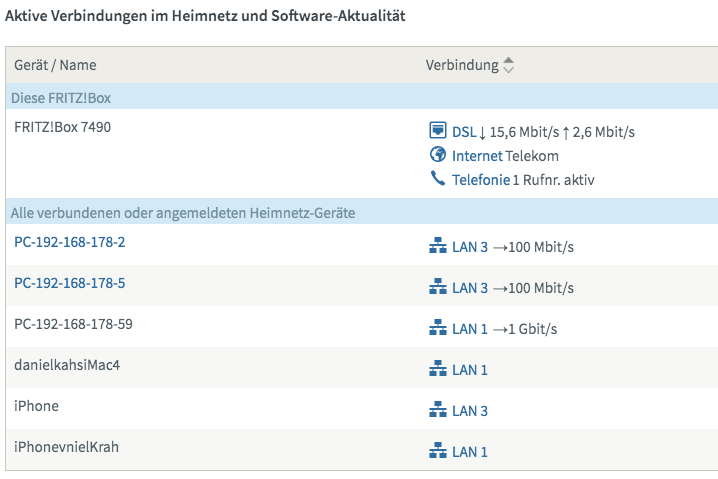
\includegraphics[scale=0.40]{./pictures/aktuelleNetzwerkGeraete.png}
\end{center}

Das ist beispielsweise beim Lan-Anschluss 3 der Fall. Hier führt ein selbst konfektioniertes Kabel mit 60 Metern parallel mit 4 Satkabeln durch mehrere Kellerräume in den Dachboden zu 2 weiteren Wlan-Routern. Diese können zwar prinzipiell 1 Gigabit/s übertragen, können aber nicht erfolgreich synchronisieren was für deren Nutzung/Funktion aber keine Rolle spielt. \\

\quote{PC-192-168-178-59} ist der Ubiquity Unify AC Pro welcher das Wlan im genutzten Zimmer bereit stellt.

% {\vspace{0.2cm}}
\begin{center}
  % \textbf{DSL-Informationen der FritzBox} (ADSL 2+ = VDSL)\\
  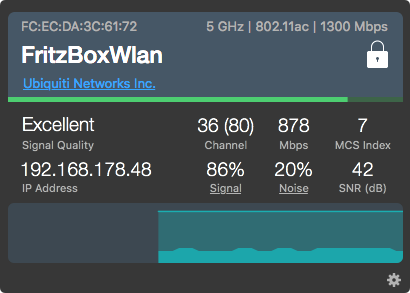
\includegraphics[scale=0.5]{./pictures/wlanSynced.png}
\end{center}

Synchronisiert wird bei 1300 Mbit/s und es stehen leicht schwankend ca. 878 Mbit/s für Nutzdaten zur Verfügung.
Von daher ist hier auch nicht mit Engpässen zu rechnen.


\newpage
\subsub{Überprüfen der Verbindung zwischen DSL-Router und Vermittlungsstelle}

Wenn eine fehlerfreie Verbindung zum Router sichergestellt ist folgt als nächstes die Überprüfung und Konfiguration der Verbindung zwischen Router und Vermittlungsstelle. \\

{\vspace{-0.1cm}}
\begin{center}
  \textbf{DSL-Informationen der FritzBox} (ADSL 2+ = VDSL)\\
  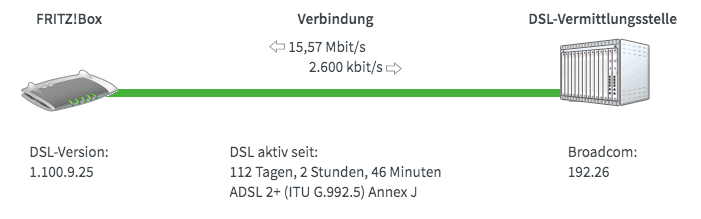
\includegraphics[scale=0.50]{./pictures/dslinfo.png}
\end{center}
Das entspricht in etwa dem gebuchten Tarif ist also ok.\\

{\vspace{-0.1cm}}
\begin{center}
  \textbf{Einstellen der Fehlerkorrektur (Störsicherheit)}\\
  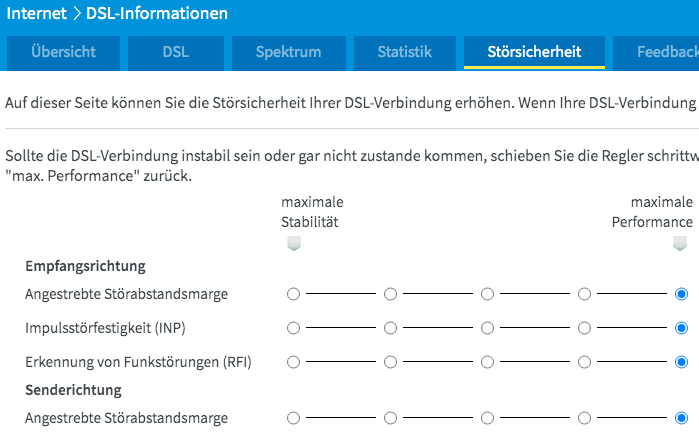
\includegraphics[width=\textwidth]{./pictures/stoersicherheit.png}
\end{center}
% 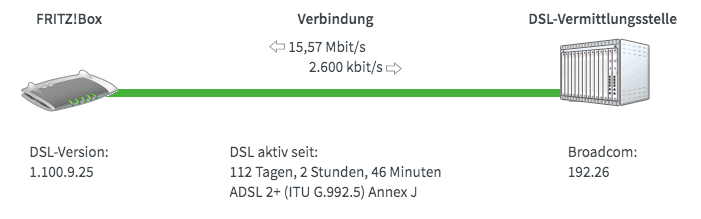
\includegraphics[width=\textwidth]{./pictures/dslinfo.png}

\newpage

Für Streaming ist es wichtig das die Daten in Echtzeit übertragen werden.
Wenn Übertragungsfehler auftreten ergibt es bei Live-Streaming keinen Sinn die Daten erneut zu senden.


{\vspace{-0.1cm}}
\begin{center}
  \textbf{Verbindungs-Informationen}\\
  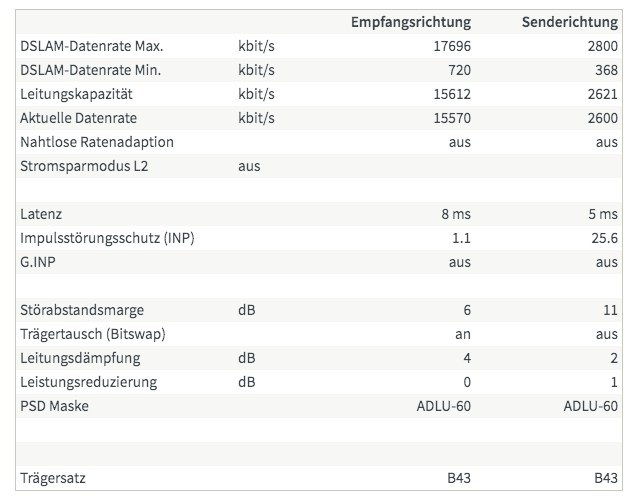
\includegraphics[scale=0.50]{./pictures/leitungsinformation.png}
\end{center}

{\vspace{-0.1cm}}
\begin{center}
  \textbf{Übertragungsfehler-Informationen}\\
  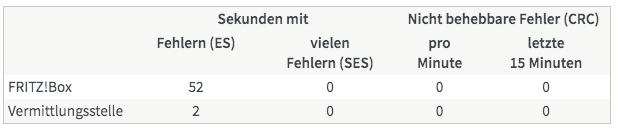
\includegraphics[scale=0.50]{./pictures/leitungsinformationFehler.png}
\end{center}

54 Fehler in 112 Tagen kann man vernachlässigen. Sollten diese innerhalb von Minuten hoch zählen sollte man die Regler nach links verschieben.
Dies drosselt dann die Verbindung wie beim Heimnetz herunter. Hier muss man das aber manuell tun und geschieht nicht automatisch.\\

Nun kann man eine zufällige Verbindung zu einem Server z.B über \quote{speedtest.net} im Internet testen.
\begin{center}
  \textbf{Ergebnis des Geschwindigkeitstest mittels Webseite} \\
  {\vspace{0.3cm}}
  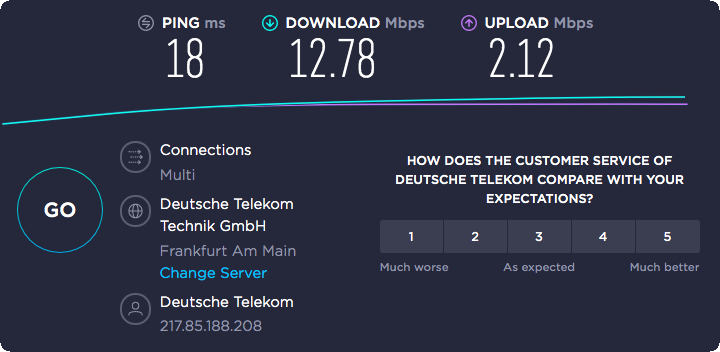
\includegraphics[scale=0.45]{./pictures/speedtestWeb.png}
\end{center}

Das entspricht dem was einem die Telekom in der Leistungsbeschreibung minimal garantiert.

Als Gegenprobe kann man den Test auch noch über das Terminal ausführen. \\

\monocodebox{sh}{Speedtest mittels Terminal:}{./codesnippets/speedtest.sh}{false}{0}{9999999}

Hier wurden ähnliche Ergebnisse erreicht, man sollte also 12 Mbit/s im Download und 2 Mbit im Upload als gegeben ansehen.



\subsub{Streaming über Youtube}

Youtube gibt, als Voraussetzung beim streamen mit einem Mobiltelefon, an das ein Stream etwa 10MB pro Minute verbraucht. \\
Eine Angabe bei welcher Auflösung und Bitrate dies der Fall ist sucht man vergebens. \\

\begin{tcolorbox}[colback=fulda_green!50!white,colframe=fulda_green,title=Berechnung der benötigten Datenrate]
  10MB * 8 (bit) : 60 (Sekunden)= \textasciitilde 13,3 Mbit/s
\end{tcolorbox}
Wenn man per Handy streamt wird ein Stromverbrauch vom 1\% pro Minute angegeben. Auch hier wird nicht darauf einegangen welches Mobiltelefon verwendet wird.
Also muss man sich sinnvolle Werte selber aus weiteren Quellen suchen oder selbst ausloten. \\

Erwünschenswert für ein Filmfestival ist eine Auflösung von 1080p. \\
Prinzipiell reichen hier 30 Bilder pro Sekunde aus, je nach Film können aber auch 60 Bilder von Vorteil sein. \\
So senden die öffentlich rechtlichen Sender wie ARD und ZDF in 720p50 da hier 50 Vollbilder pro Sekunde möglich sind. Die Sendeanstalten begründen diese Wahl damit, dass diese Auflösungs/Bildwiederholfrequenz Kombination insbesondere bei Sportveranstaltungen, bei denen schnelle Bewegungen vorkommen, von Vorteil ist.\\
Ansonsten könnten Sie nur in 1080i senden, welches über Satellit nur mit 24 oder 30 Vollbildern, sowie 60 Halbbildern im Zeilensprungverfahren möglich ist.
Man spart, mit ca 46,1 Mpx/s im Gegensatz zu 62,2 Mpx/s bei 1080p30/i60, auch etwas an Daten welche übertragen werden müssen.\\

Bei der Übertragung über das Internet spielt dies bei einer Flatrate aber keine Rolle. \\
Außer man streamed über seinen Mobilfunkvertrag oder beispielsweise über das Netz der Universität Darmstadt, da diese nicht am DFN hängen und für ihren Datenverkehr bezahlen müssen.

\subsub{Welche Datenrate wird bei welcher Auflösung benötigt?}

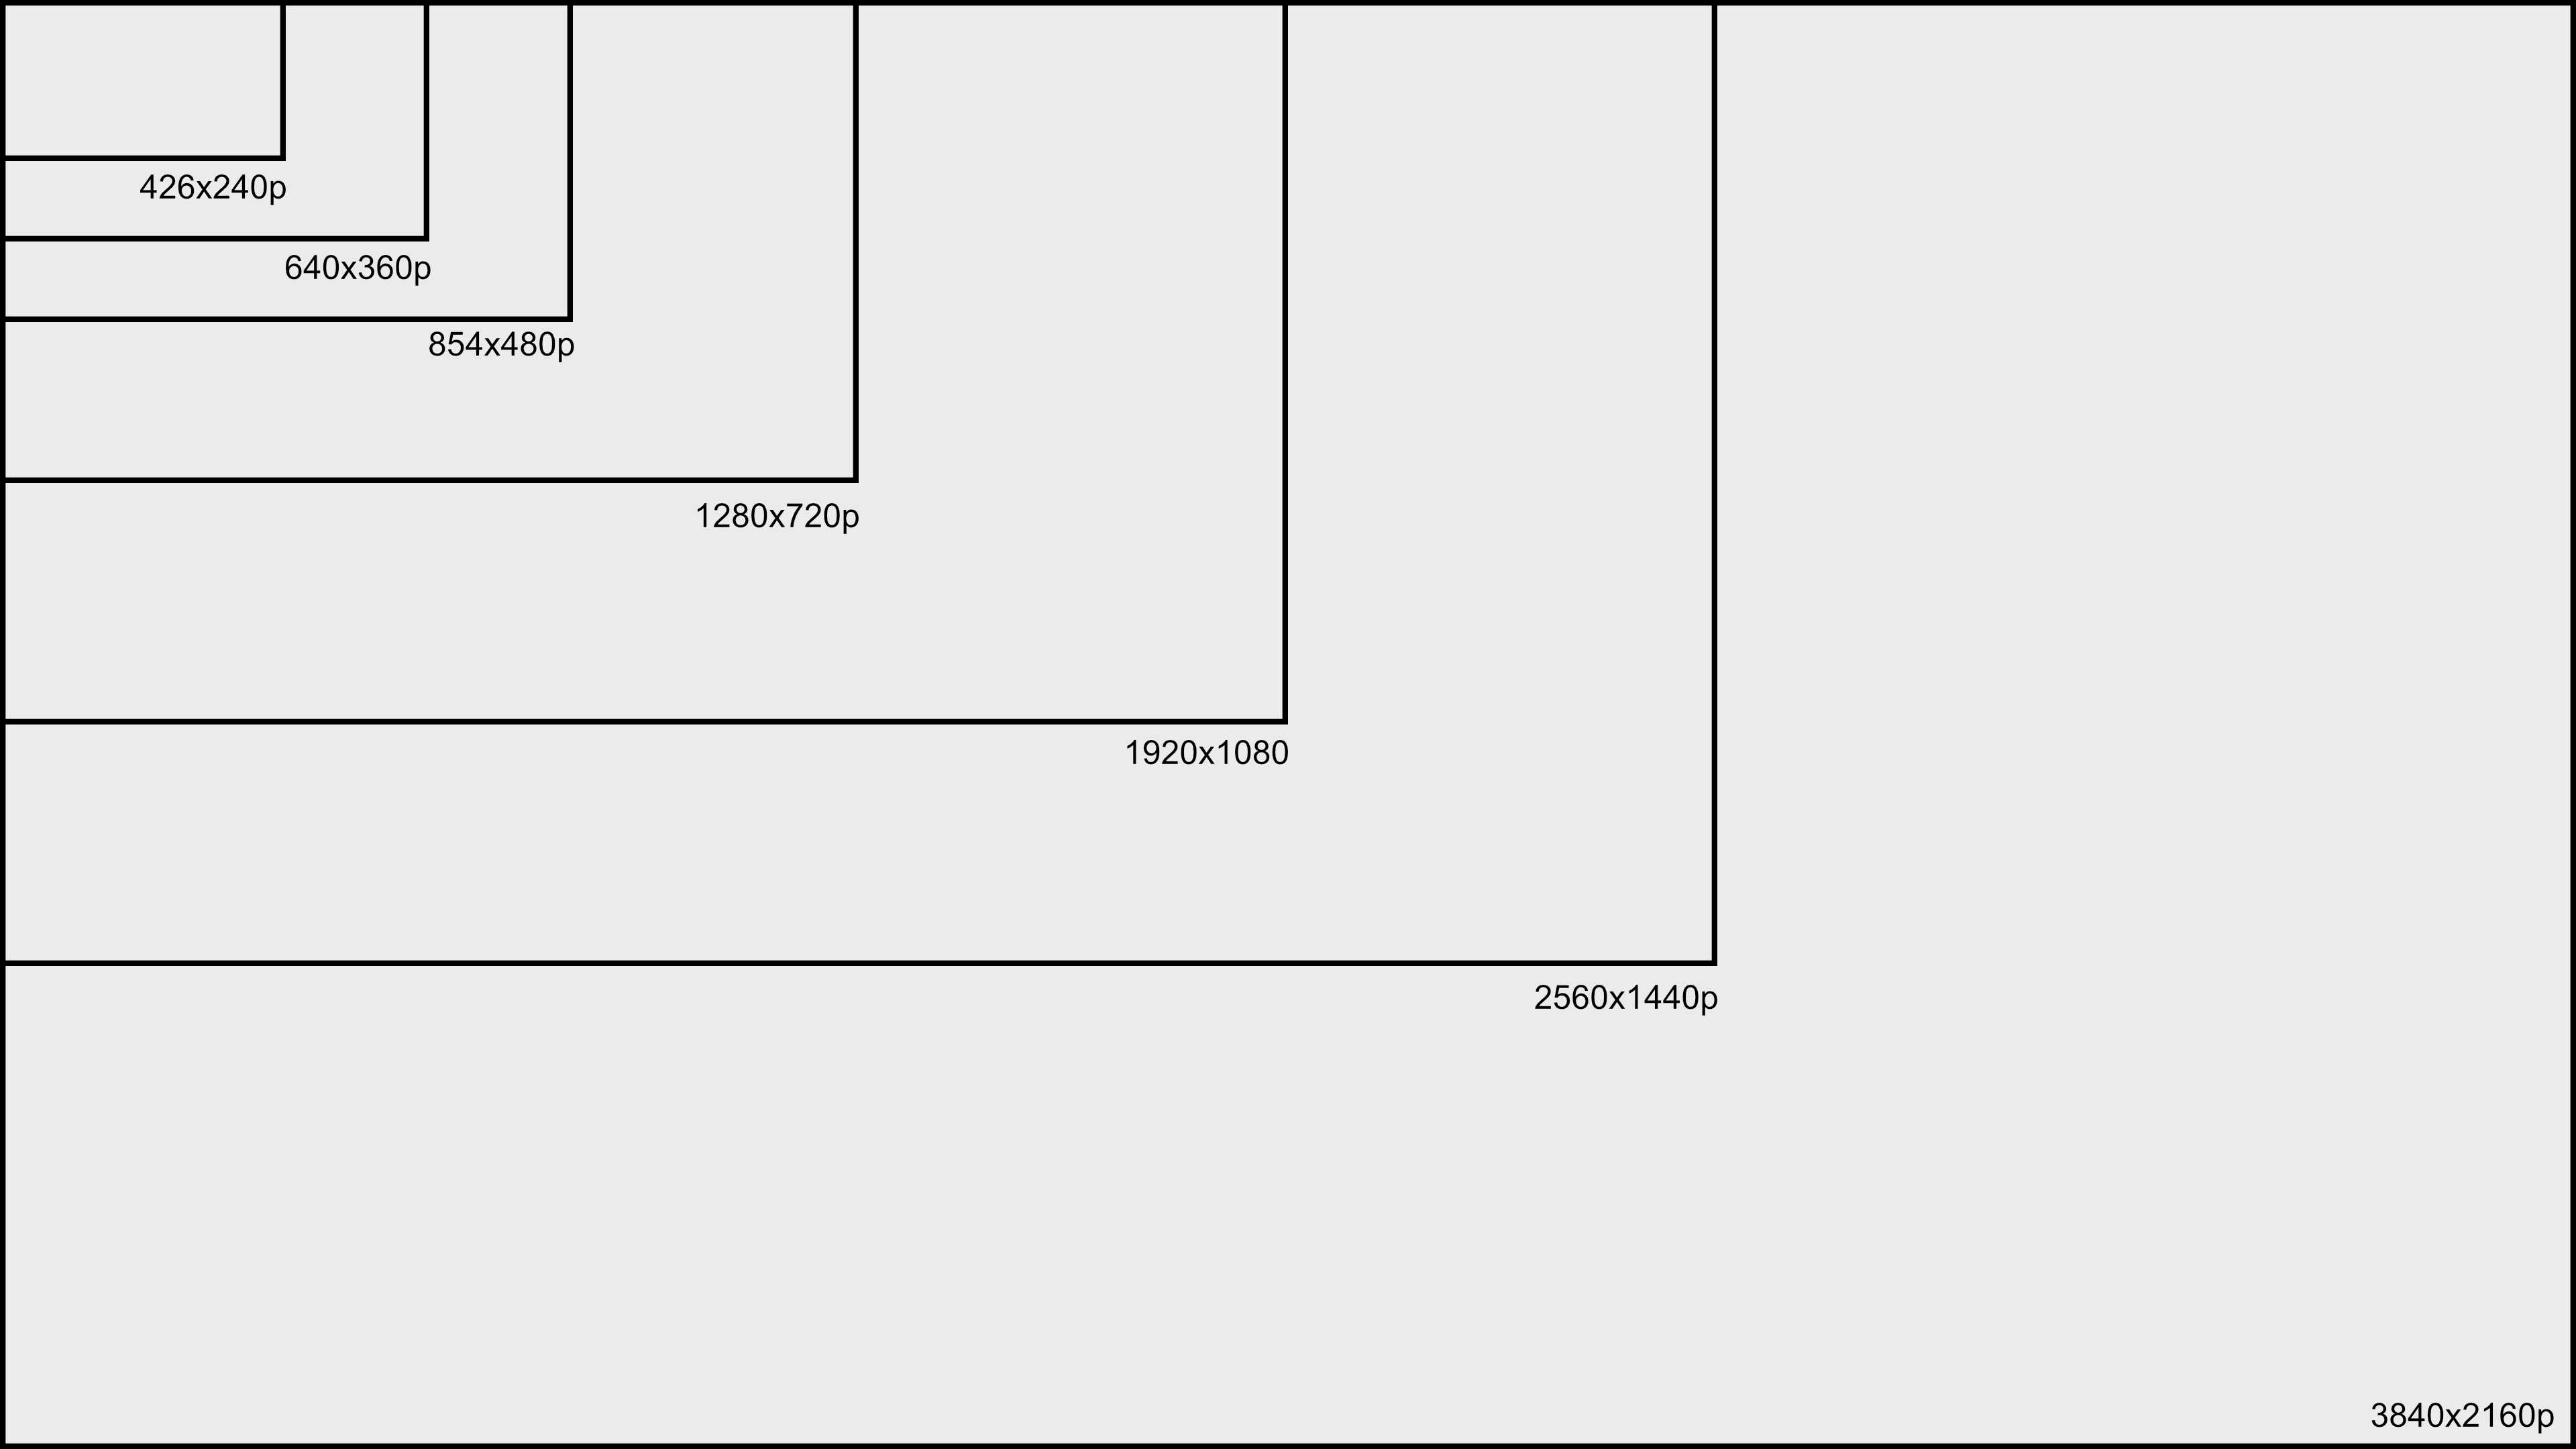
\includegraphics[width=\textwidth]{./pictures/resolutions.png}

\begin{center}
  \textbf{Empfohlene Datenraten für Youtube}
  \begin{table}[ht]
    \begin{tabular}{|>{\raggedleft}p{1,6cm} >{\raggedleft}p{1,9cm}| >{\centering}p{1,4cm}| >{\raggedleft}p{0,9cm}>{\raggedleft}p{0,1cm} >{\raggedleft}p{2,07cm}|  >{\centering}p{2,3cm}| >{\centering}p{2,8cm}|}   % \begin{tabular}*{5}{|c}      %
      \hline
      \rowcolor{fulda_green}
      \multicolumn{2}{|c|}{Auflösung}   &  Bildrate     & \multicolumn{3}{|c|}{Video-Bitrate in kbit/s}         &  Audio-Bitrate    & Minimaler Upload Mbit   \tabularnewline  \hline  \hline  \rowcolor{fulda_green!66}
      4k/2160p  & 3.840x2.160p          & 60            & 20.000 & – & 51.000 kbit/s    & 128 kbits/s       & 40.2 Mbit/s            \tabularnewline  \hline  \rowcolor{fulda_green!33}
      4k/2160p  & 3.840x2.160p          & 30            & 13.000 & – & 34.000 kbit/s    & 128 kbits/s       & 26.2 Mbit/s            \tabularnewline  \hline  \rowcolor{fulda_green!66}
      1440p     & 2.560x1.440p          & 60            & 9.000 & – & 18.000 kbit/s     & 128 kbits/s       & 18.2 Mbit/s            \tabularnewline  \hline \rowcolor{fulda_green!33}
      1440p     & 2.560x1.440p          & 30            & 6.000 & – & 13.000 kbit/s     & 128 kbits/s       & 12.2 Mbit/s            \tabularnewline  \hline  \rowcolor{fulda_green!66}
      1080p     & 1.920x1.080p          & 60            & 4.500 & – & 9.000 kbit/s      & 128 kbits/s       & 9.2 Mbit/s             \tabularnewline  \hline \rowcolor{fulda_green!33}
      1080p     & 1.920x1.080p          & 30            & 3.000 & – & 6.000 kbit/s      & 128 kbits/s       & 6.2 Mbit/s             \tabularnewline  \hline  \rowcolor{fulda_green!66}
      720p      & 1.280x720p            & 60            & 2.250 & – & 6.000 kbit/s      & 128 kbits/s       & 4.7 Mbit/s             \tabularnewline  \hline \rowcolor{fulda_green!33}
      720p      & 1.280x720p            & 30            & 1.500 & – & 4.000 kbit/s      & 128 kbits/s       & 3.2 Mbit/s             \tabularnewline  \hline  \rowcolor{fulda_green!66}
      480p      & 854x480p              & 30            & 500 & – & 2.000 kbit/s        & 128 kbits/s       & 1.2 Mbit/s             \tabularnewline  \hline \rowcolor{fulda_green!33}
      360p      & 640x360p              & 30            & 400 & – & 1.000 kbit/s        & 128 kbits/s       & 1 Mbit/s               \tabularnewline  \hline  \rowcolor{fulda_green!66}
      240p      & 426x240p              & 30            &  300 & – & 700 kbit/s         & 128 kbits/s       & 0.8 Mbit/s              \tabularnewline  \hline \rowcolor{fulda_green!33}
    \end{tabular}
  \end{table}
\end{center}

Im oberen Bild sieht man einen Größenvergleich der einzelnen Videoauflösungen. In der unteren Tabelle sind empfohlene Datenraten basierend aus Informationen verschiedenster Foren sowie sozialer Netzwerke. \\

Bei der Videobitrate ist der Minimalwert immer so hoch damit das Bild eine akzeptable Qualität hat. Beim Maximalwert ist kein Qualitätsverlust sichtbar.
Da es bei der Datenübertragung immer zu Schwankungen kommen kann, beispielsweise wenn: \quote{Abends alle Netflix schauen} , sollte man einen Puffer einplanen. Pi mal Daumen nimmt man die minimale Datenrate mal 2 und addiert die Tondatenrate, aufgerundet auf die nächste 100er Stelle, auf. \\

\newpage
So kann, es wie man sieht, bei einem DSL 50 Vertrag über Fiber bei 1080p60 \\
schon knapp werden. Im schlimmsten Fall steht man beim Upload nicht viel besser da als mit meinem DSL 16 Vertrag, wenn der Upload komplett über die störungsanfälligere VDSL Technologie übertragen wird und nicht wie bei Fiber to the curb, zumindest auf einer Teilstrecke, über Glasfaser. \\

Während man so über FTTC relativ sicher kalkulieren kann, sollte man bei reiner VDSL Technik für 1080p mindestens DSL 100 buchen.\\

1440p60 sollte über Kupfer VDSL grade so noch gehen, für 4K Streams benötigt aber mindestens FTTC mit DSL 100 oder besser einen direkten Glasfaseranschluss.


\subsub{Latenz}

Wenn man eine Moderation und/oder Livechat nutzen möchte, sollte man sich auch mit den Latenzen beschäftigen.

So empfehlen einige Youtuber für 1080p-Streams:
\begin{itemize}
  \item Normale Latenz: \textasciitilde 6-10 Mbit/s
  \item Niedrige Latenz: \textasciitilde 5-6 Mbit/s
  \item Sehr niedrige Latenz: \textasciitilde 4,5-5 Mbit/s
\end{itemize}

Letztere ist wichtig wenn man Echtzeitkommunikation mit den Zuschauern halten möchte, ansonsten kann es zu Verzögerungen von 5 Sekunden und auch deutlich mehr im Chat kommen.

\subsub{Exkurs zu anderen Plattformen}

Bei Twitch kann man wenn man nicht Twitch-Partner ist langfristig höchstens mit 720p und einer Datenrate von 3-3,5 Mbit/s streamen.

Bei anderen Webseiten welche Livestreaming anbieten sieht es ähnlich aus.\\
Facebook (720P @ \textasciitilde 4 Mbit/s) \\
Mixer (720P @ \textasciitilde 6 Mbit/s) \\

Twitch und Mixer unterstützen, wenn man kein Partner ist, kein downscaling.
Das bedeutet das wenn man auf seinem Mobiltelefon und LTE einen Stream schauen möchte, nur 720p zur Verfügung hat und nicht auf 360p umschwenken kann um sein Datenvolumen zu schonen. \\

Mixer, welcher ein Dienst von Microsoft war, wurde am 23. Juli 2020 geschlossen.


\newpage

\sub{Verwendete Hardware für Streamingtests}

Für Streamingtests stehen verschiedene Geräte zur Verfügung.\\

2x iPhone SE, 1x iPhone6, Ein Macbook Pro \zoll{15} late 2015, sowie ein Eigenbau Mac (Hackintosh).\\
Die iPhones werden nicht verwendet, obwohl diese zwar prinzipiell für den geplanten Einsatz geeignet sind, aber zu umständlich in der Bedienung wären.\\

Das Haus ist schon im vorigen Kapitel erwähnt auf den wichtigsten Strecken mit Gigabit verkabelt und als Wlan-Router wird ein Ubiquiti AC PRO verwendet,
welcher 450 Mbit bei 2,4 GHz und 1300 Mbit (\quote{Netto} \textasciitilde 850 Mbit/s) bei 5 GHz an Übertragungskapazität zur Verfügung stellt.
Der DSL-Router ist eine FritzBox 7490 welcher noch von der Rhön Energie stammt.
Engpässe können daher innerhalb des Hauses wie schon festgestellt nicht auftreten.



% {\vspace{-2cm}}
\subsub{Eigenbau Mac}
Standard Windows-PC mit Clover-Bootloader um MacOS starten zu können.
\small
\color{black}
\vspace{0.3cm}
\begin{center}
  \begin{tikzpicture}
    \clip node (m) [matrix,matrix of nodes,
    fill=fulda_green!20,inner sep=0pt,
    nodes in empty cells,
    nodes={minimum height=1cm,minimum width=2.6cm,anchor=center,outer sep=0,font=\sffamily},
    row 1/.style={nodes={fill=fulda_green,text=white}},
    column 1/.style={nodes={fill=fulda_green,text=white,align=left,text width=3cm,text depth=0.5ex}},
    column 2/.style={text width=12cm,align=left,every even row/.style={nodes={fill=white}}},
    column 3/.style={text width=3cm,align=center,every even row/.style={nodes={fill=white}},},
    row 1 column 1/.style={nodes={fill=fulda_green}},%									1. spalte oben
    prefix after command={[rounded corners=4mm] (m.north east) rectangle (m.south west)}
    ] {
    & $\ \ $ Hackintosh Gigabyte Z77 DS3H Mainboard\\
    $\ \ $ CPU, RAM   			& $\ \ $ i7 3770, 24 GB\\
    $\ \ $ FESTPLATTE				& $\ \ $ 240GB PCIE, 92TB SATA\\
    $\ \ $ WAN/LAN		& $\ \ $ Atheros Gigabit Netzwerk \\
    $\ \ $ WIFI		    & $\ \ $ TP-Link T8E  450/1300 Mbit AC Wifi \\
    $\ \ $ USB				& $\ \ $ V2.0 / v3.0	 \\
    $\ \ $ MONITOR		& $\ \ $ \zoll{27} Samsung SMS27A650\\
    & $\ \ $ \zoll{24} Samsung SyncMaster \\
    & $\ \ $ \zoll{15} iiyama 4:3 \\
    $\ \ $ KAMERA			& $\ \ $ Logitech C270, Logitech C310  \\
    $\ \ $ MIKROFON 	& $\ \ $ RØDE NT-USB  \\
    $\ \ $ OS 			& $\ \ $ MacOS 10.13 High Sierra \\
    };
  \end{tikzpicture}
\end{center}
\normalsize

\newpage
% {\vspace{-0,5cm}}
\subsub{Apple Macbook Pro Retina 15\grqq{} late 2015 }

Standard Macbook Pro Retina in Vollausstattung.\\
Die SSD wurde ausgetauscht als 80\% der zu erwartenden Schreibzyklen aufgebraucht waren.
%
\small
\color{black}
\vspace{0.3cm}
\begin{center}
  \begin{tikzpicture}
    \clip node (m) [matrix,matrix of nodes,
    fill=fulda_green!20,inner sep=0pt,
    nodes in empty cells,
    nodes={minimum height=1cm,minimum width=2.6cm,anchor=center,outer sep=0,font=\sffamily},
    row 1/.style={nodes={fill=fulda_green,text=white}},
    column 1/.style={nodes={fill=fulda_green,text=white,align=left,text width=3cm,text depth=0.5ex}},
    column 2/.style={text width=12cm,align=left,every even row/.style={nodes={fill=white}}},
    column 3/.style={text width=3cm,align=center,every even row/.style={nodes={fill=white}},},
    row 1 column 1/.style={nodes={fill=fulda_green}},%									1. spalte oben
    prefix after command={[rounded corners=4mm] (m.north east) rectangle (m.south west)}
    ] {
    & $\ \ $ Apple Macbook Pro Retina \zoll{15}\\
    $\ \ $ CPU, RAM   			& $\ \ $ i7 4870HQ, 16 GB\\
    $\ \ $ FESTPLATTE 				& $\ \ $ 1TB PCIE (nachgerüstet, langsamer als die originale SSD welche Defekt war)  \\
    $\ \ $ WAN/LAN		& $\ \ $ Thunderbolt Gigabit Adapter \\
    $\ \ $ WIFI		    & $\ \ $ Integriertes 600/1300 Mbit AC Wifi \\
    $\ \ $ USB				& $\ \ $ v3.0	 \\
    $\ \ $ MONITOR		& $\ \ $ integriertes \zoll{15} Retina Display	 \\
    $\ \ $ KAMERA			& $\ \ $ Logitech C270 (mehrere vorhanden)  \\
    $\ \ $ MIKROFON 	& $\ \ $ Integriert oder RØDE NT-USB  \\
    $\ \ $ OS 			  & $\ \ $ MacOS 10.14 Mojave \\
    };
  \end{tikzpicture}
\end{center}
\normalsize

{\vspace{0.5cm}}

Da beide Computer ähnlich ausgestattet sind verwendete ich für Streamingtest aus Bequemlichkeit und da dieser stabiler \quote{läuft} den Hackintosh.
Ebenso habe ich an diesen schon mehrere Monitor fest angeschlossen.


\subsub{Genutzte Streamingsoftware}
% {\vspace{-0.6cm}}
\begin{center}
  \textbf{Streamingprogramme} \\
  
\includegraphics[scale=0.35]{./pictures/streamlabsOBJ.png}
\end{center}



\begin{itemize}
  \item OBS
  \item Streamlabs OBS
  \item Webbrowser (Vivaldi Chrome basierend)
\end{itemize}




%
% Eigenbau mit MacOS 10.13.

% \small
% \color{black}
% \vspace{0.3cm}
% \begin{center}
% \begin{tikzpicture}
% \clip node (m) [matrix,matrix of nodes,
% fill=fulda_green!20,inner sep=0pt,
% nodes in empty cells,
% nodes={minimum height=1cm,minimum width=2.6cm,anchor=center,outer sep=0,font=\sffamily},
% row 1/.style={nodes={fill=fulda_green,text=white}},
% column 1/.style={nodes={fill=fulda_green,text=white,align=left,text width=3cm,text depth=0.5ex}},
% column 2/.style={text width=12cm,align=left,every even row/.style={nodes={fill=white}}},
% column 3/.style={text width=3cm,align=center,every even row/.style={nodes={fill=white}},},
% row 1 column 1/.style={nodes={fill=fulda_green}},%									1. spalte oben
% prefix after command={[rounded corners=4mm] (m.north east) rectangle (m.south west)}
% ] {
% & $\ \ $ Iphone SE\\
% $\ \ $ CPU   			& $\ \ $ Apple A9 2x 1.85 GHz\\
% $\ \ $ RAM 				& $\ \ $ 2 GB LPDDR4 \\
% $\ \ $ WIFI		    & $\ \ $ Broadcom AC Wifi 433 Mbit \\
% $\ \ $ USB				& $\ \ $ v3.0	 \\
% $\ \ $ CAM		    & $\ \ $ 12 megapixels with 1.22µ pixels (iSight)	 \\
%                   & $\ \ $ 1.2 megapixels (FaceTime) \\
% $\ \ $ MICROPHONES& $\ \ $ 3x integriert	 \\
%                   & $\ \ $ 1x Extern Junlin Mikrofon \\
% $\ \ $ OS 			  & $\ \ $ latest IOS\\
% 						      & $\ \ $ 867 Mbit (2x2) im 5 Ghz Band (AC) \\
% };
% \end{tikzpicture}
% \end{center}
% \normalsize

\newpage
\sub{Zwischen-Fazit}
Da Formula Mundi ein Filmfestival ist und die Filme vorproduziert sind bieten sich Youtube Premieren an.
Mit Ihnen ist es Möglich die Filme zu zeigen und trotzdem eine Kommunikationsmöglichkeit während des Films zu haben.
Ebenso kann man auch beispielsweise 10 Minuten lang ein Bild davor und oder dahinter schneiden um dort eine Diskussion halten zu können.
Die Anmoderation kann natürlich auch als Film abgedreht sein und wird dann einfach davor geschnitten.

\sect{Vorbereitung des Streams/Premiere}

Bei einem Livestream der Premiere gibt es einiges bezüglich des Chats zu beachten:
\begin{itemize}
  \item Moderatoren sollten vor einem Chat zugewiesen sein.
  \item Blockieren von unangemessenen Wörtern oder Links aktivieren.
  \item Langsamen Modus aktivieren damit Zuschauer nicht den Chat zu spammen können.
  \item \grqq{}Zur Überprüfung zurückhalten\grqq{} aktivieren damit problematische Wörter nicht im chat erscheinen.
\end{itemize}

Ebenso muss man gegebenenfalls die Streaming-Software mit Youtube koppeln.

\newpage
\sect{OBS /OBS Studio Einrichten}

% \sub{Stream planen}

{\vspace{0.2cm}}
\begin{center}
  \textbf{Hierfür klickt hierfür auf \quote{Stream planen } rechts oben.} \\
  {\vspace{0.3cm}}
  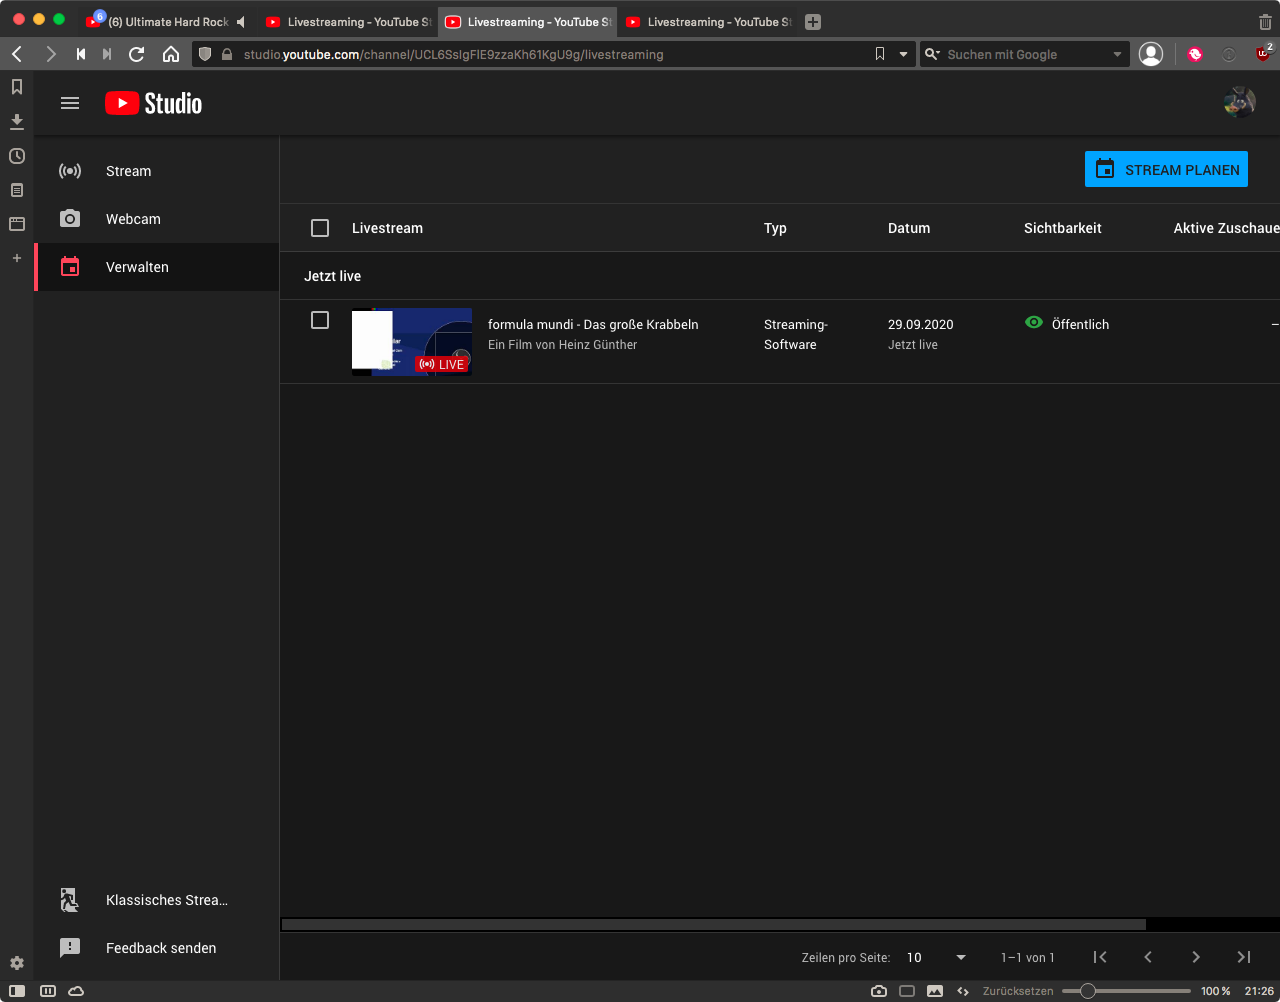
\includegraphics[width=0.7\textwidth]{./pictures/YOUTUBEstreamPlanen1.png}
\end{center}



% {\vspace{-0.6cm}}
\begin{center}
  \textbf{Hier ist es wichtig die Zielgruppeneinstellung zu setzen.} \\
  {\vspace{0.3cm}}
  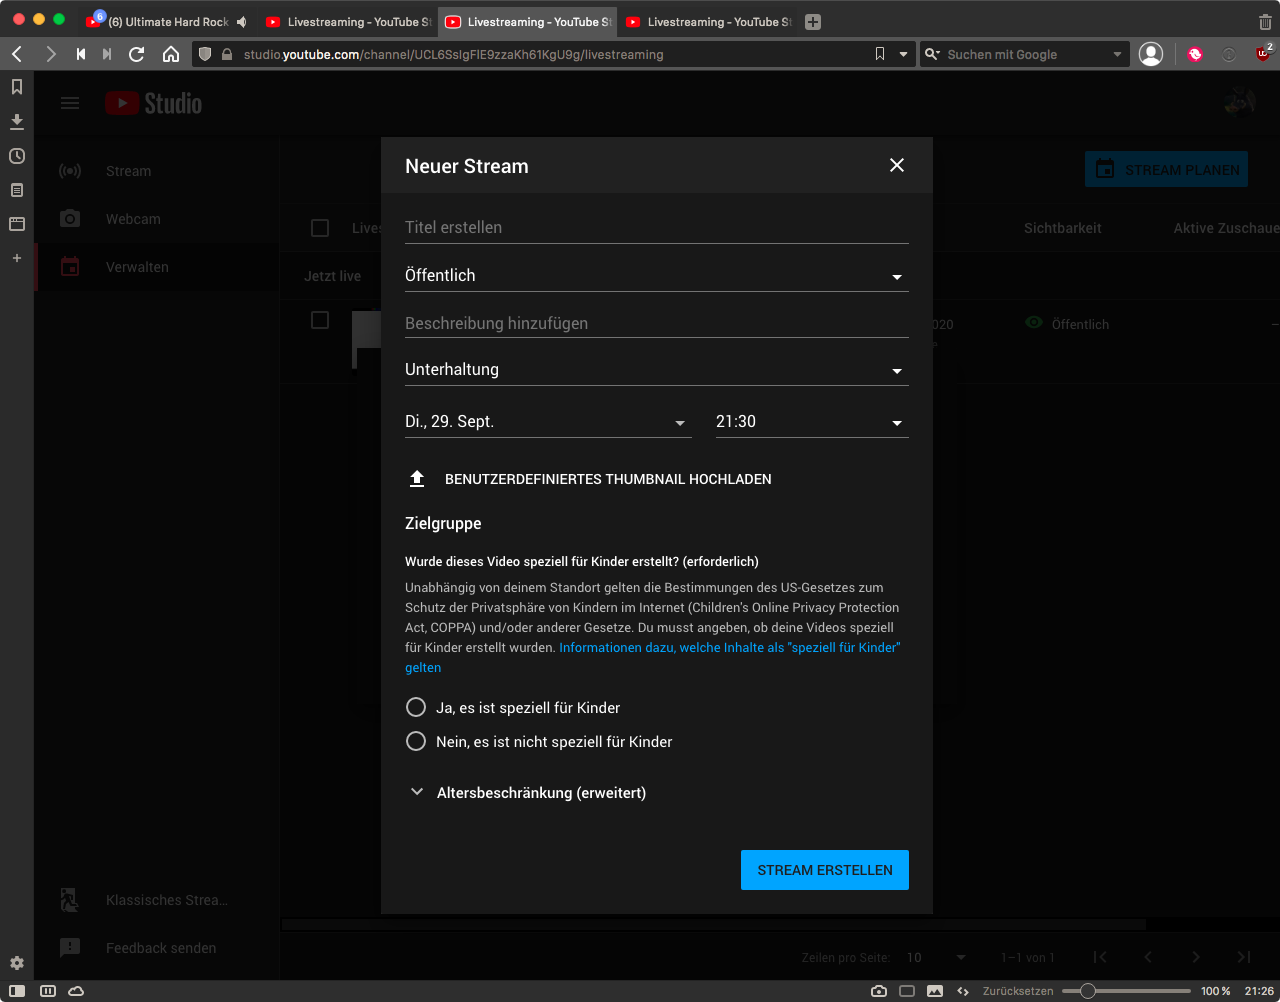
\includegraphics[width=0.7\textwidth]{./pictures/YOUTUBEstreamPlanen2.png}
\end{center}

\newpage
% {\vspace{-0.6cm}}
\begin{center}
  \textbf{In den Stream Einstellungen kann man nun die Latenz Einstellen und bekommt den Stream-Schlüssel für OBS} \\
  {\vspace{0.3cm}}
  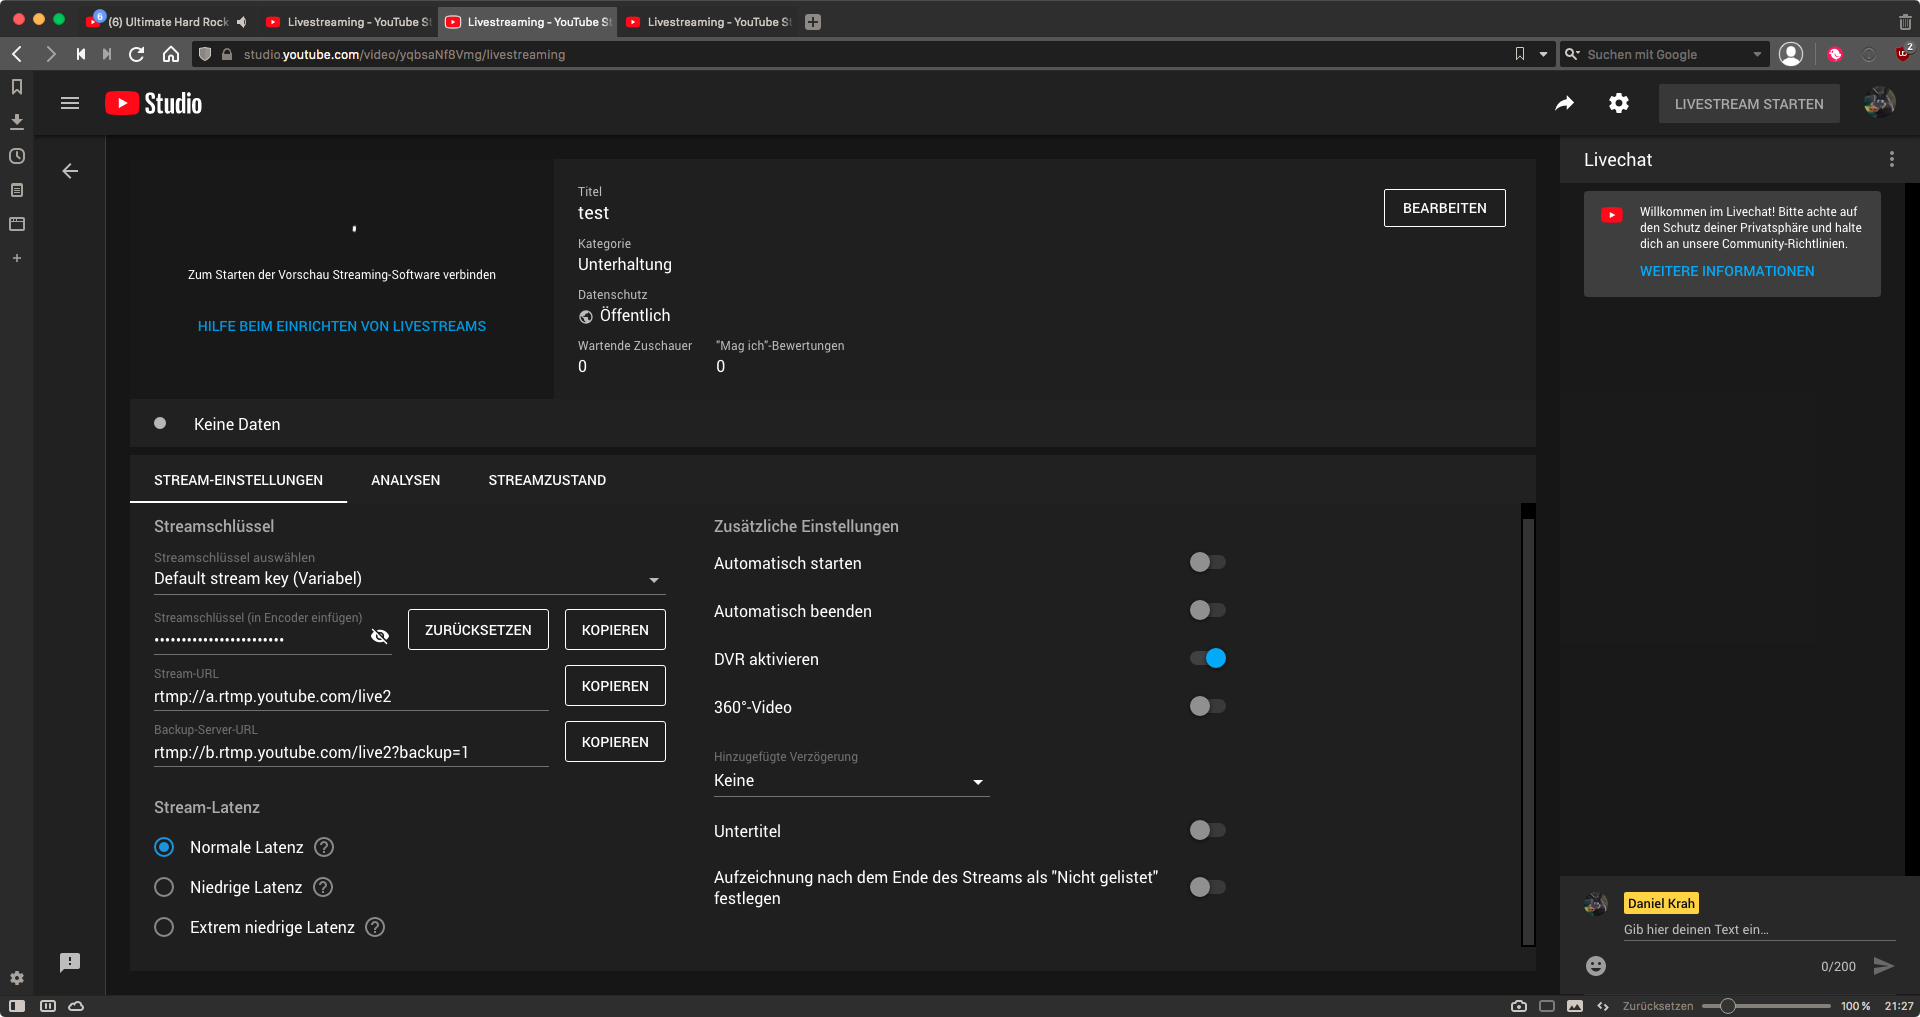
\includegraphics[width=0.9\textwidth]{./pictures/YOUTUBEstreamPlanen3.png}
\end{center}

% {\vspace{-0.6cm}}
\begin{center}
  \textbf{Diesen kann man nun in OBS unter Stream eintragen} \\
  {\vspace{0.3cm}}
  \includegraphics[width=0.7\textwidth]{./pictures/schlüsselEingetragen.png}
\end{center}

\newpage
% {\vspace{-0.6cm}}
\begin{center}
  \textbf{Es müssen als Nächstes die Datenraten für Audio und Video gesetzt werden ...} \\
  {\vspace{0.3cm}}
  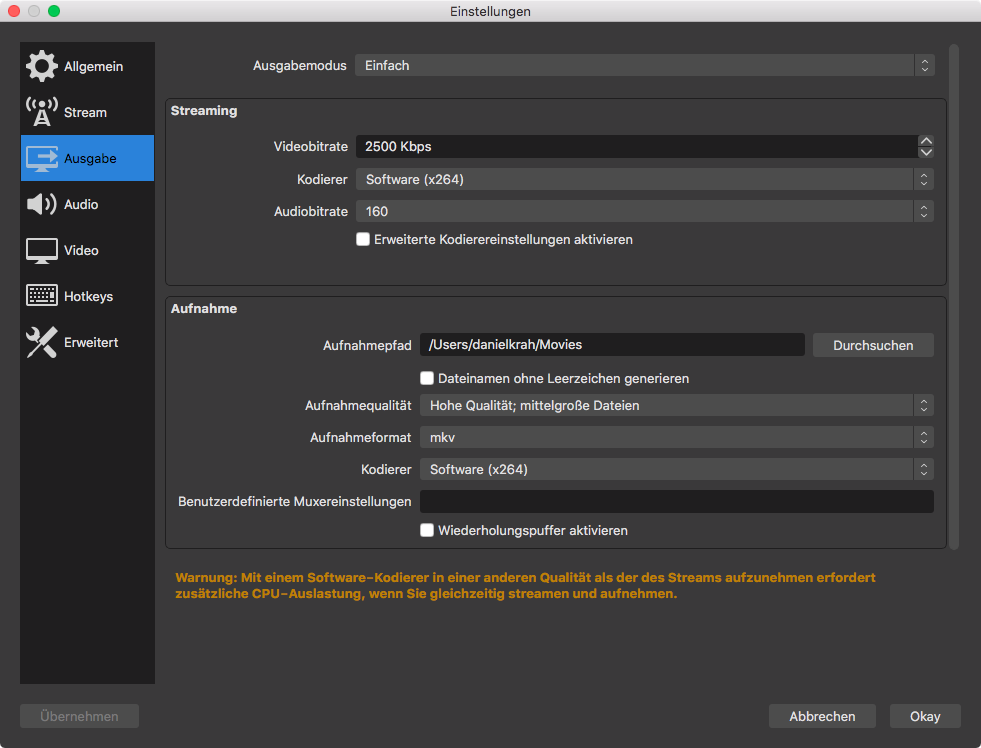
\includegraphics[width=0.7\textwidth]{./pictures/configDatenRate.png}
\end{center}

% {\vspace{-0.6cm}}
\begin{center}
  \textbf{... Sowie die Auflösung für den Videostream} \\
  {\vspace{0.3cm}}
  \includegraphics[width=0.7\textwidth]{./pictures/configAuflösung.png}
\end{center}



\newpage
% {\vspace{-0.6cm}}
\begin{center}
  \textbf{In beiden Programmen können Filme als Videoquelle sowie Webcams eingebunden werden} \\
  \textbf{Ebenso sind Hintergründe möglich.} \\
  {\vspace{0.3cm}}
  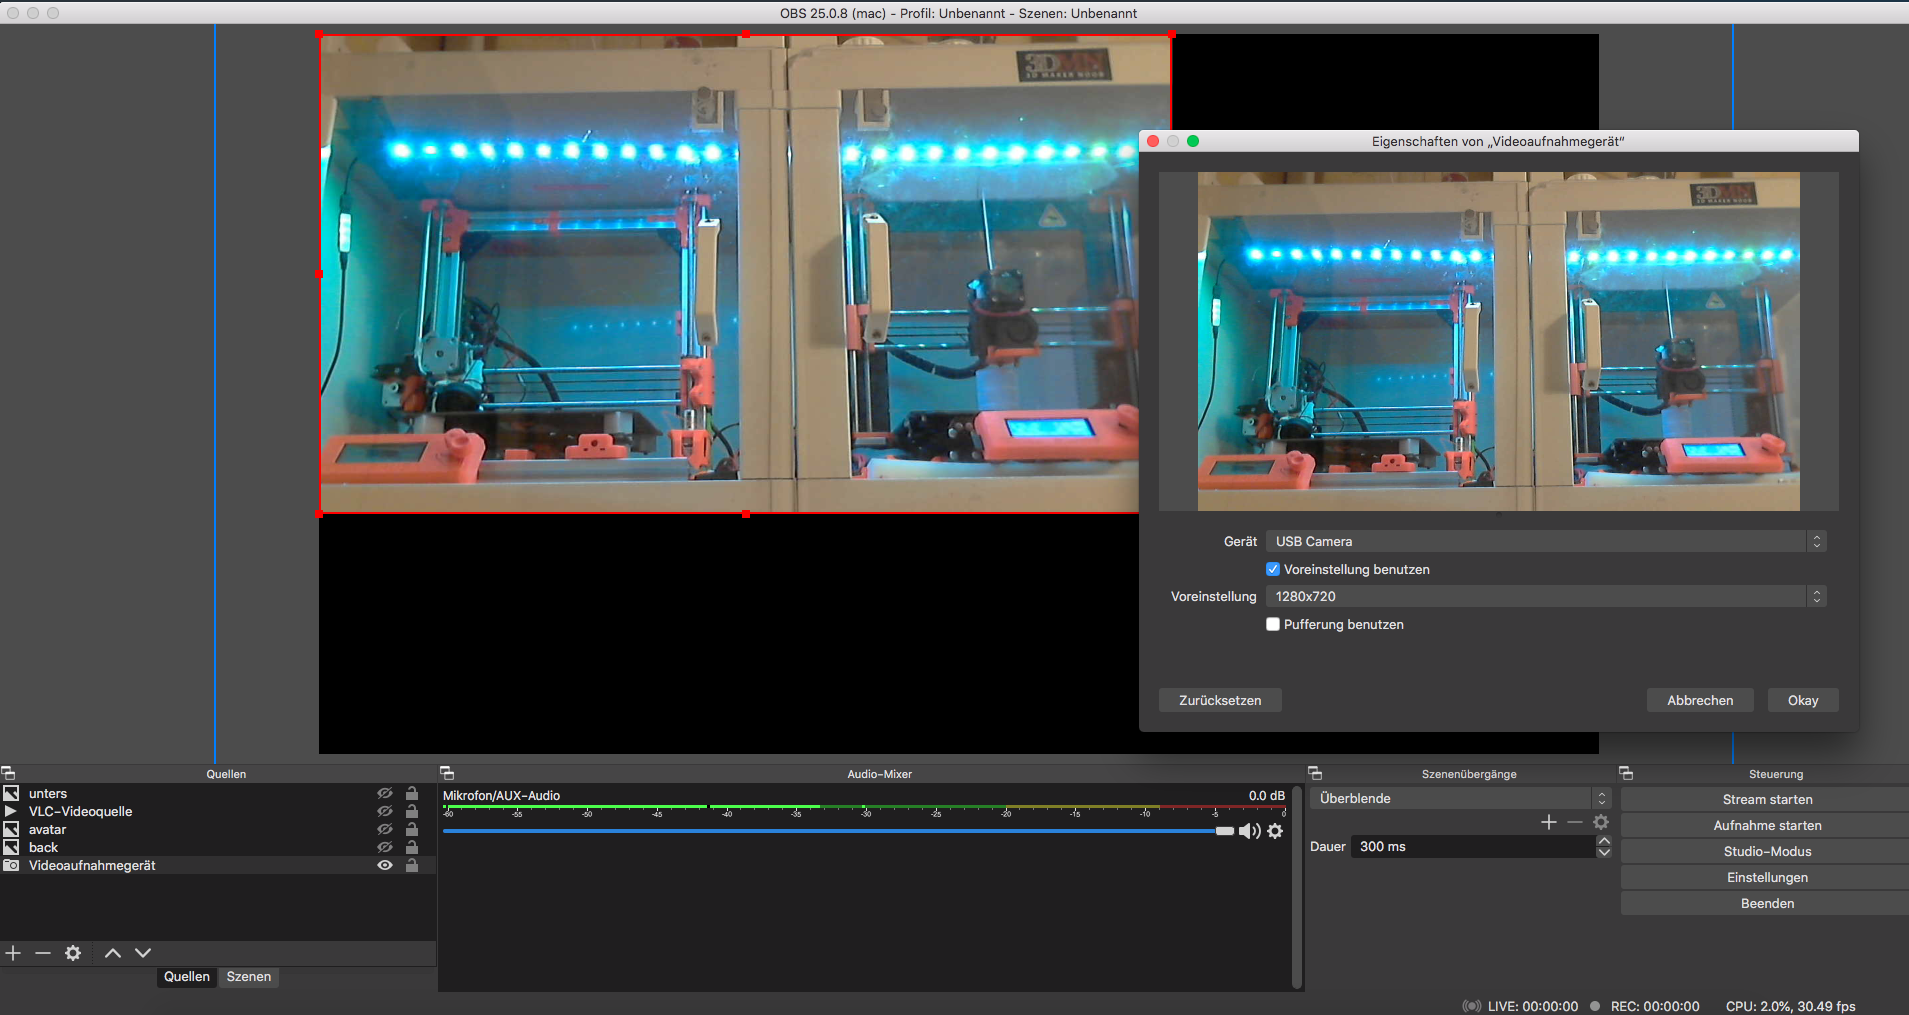
\includegraphics[width=0.9\textwidth]{./pictures/usbcamOBS.png}
\end{center}

% {\vspace{-0.6cm}}
\begin{center}
  \textbf{Hier läuft ein Film neben einem Kamera-Stream über einem Hintergrund } \\
  {\vspace{0.3cm}}
  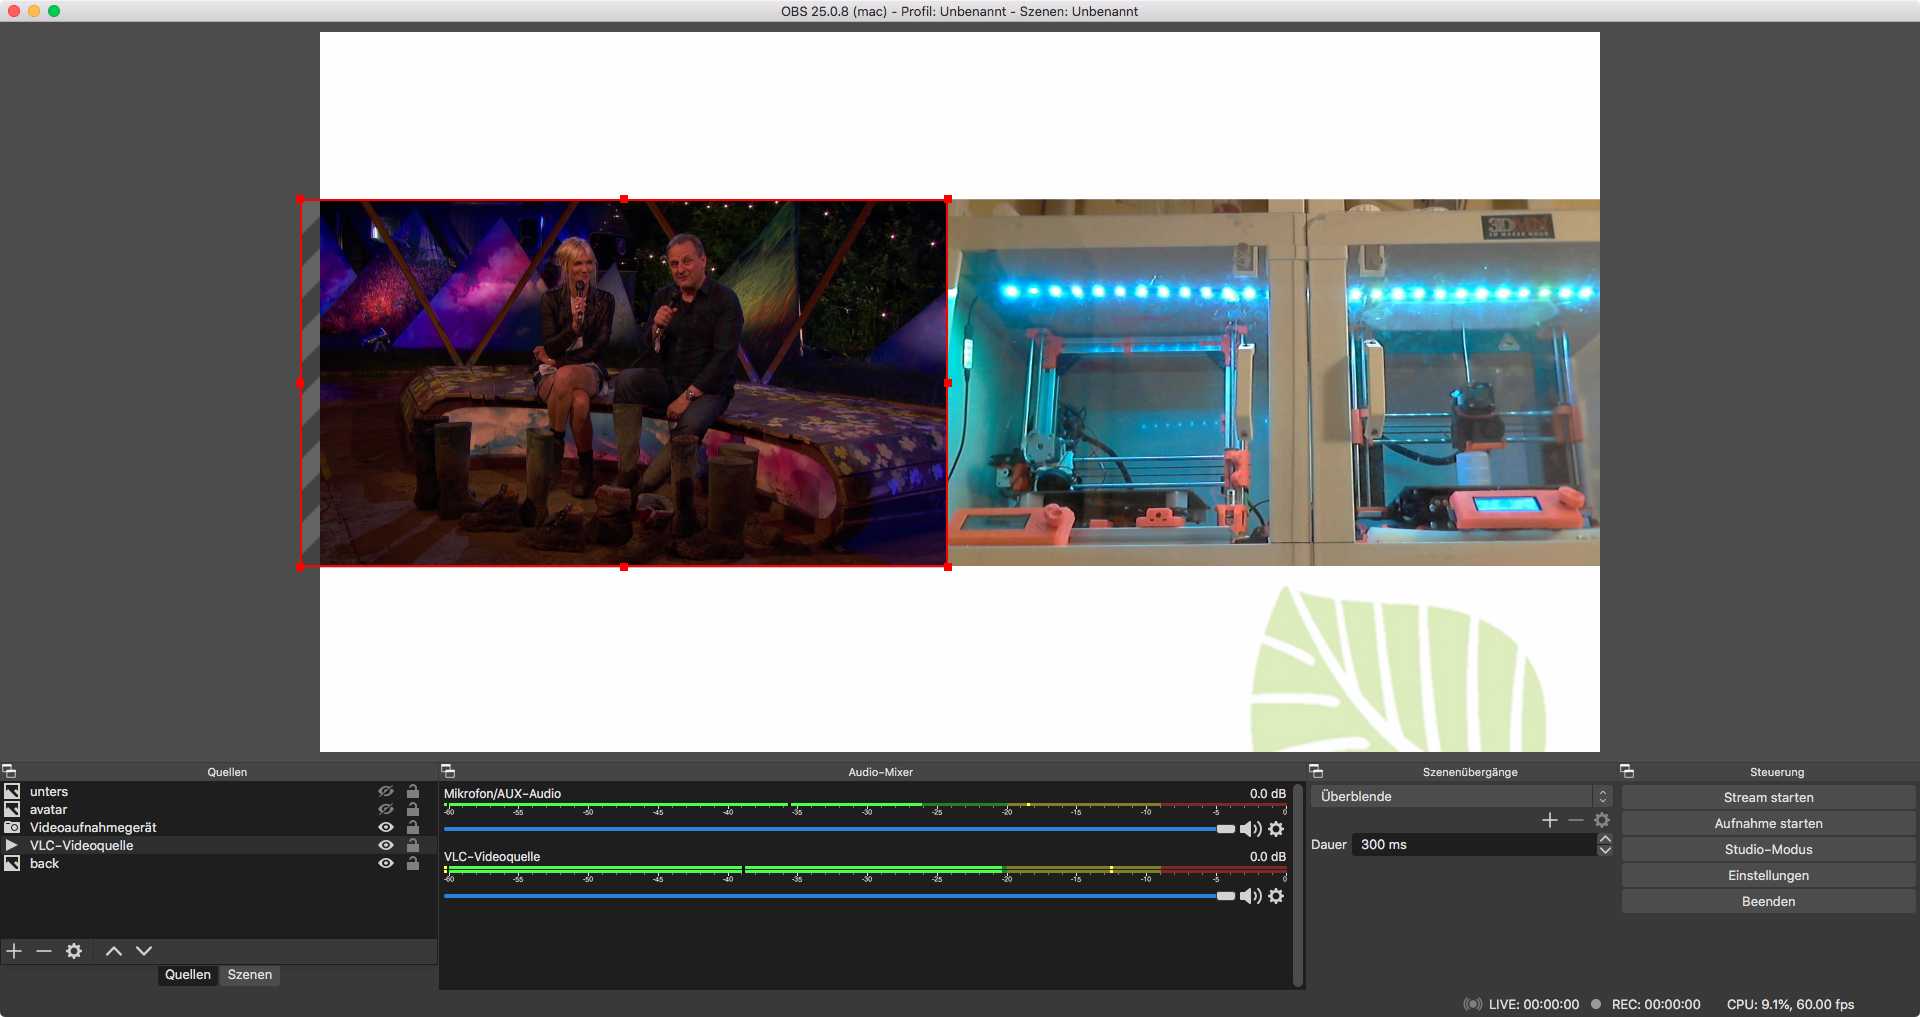
\includegraphics[width=0.7\textwidth]{./pictures/videoCAMsideBYside.png}
\end{center}

\newpage
\sect{Live-Streaming auf Youtube}

{\vspace{0.2cm}}
\begin{center}
  \textbf{Hierfür klickt hierfür auf \quote{Livestream starten } rechts oben.} \\
  \textbf{(Dies setzt voraus das OBS mit Youtube verbunden ist.)} \\
  {\vspace{0.3cm}}
  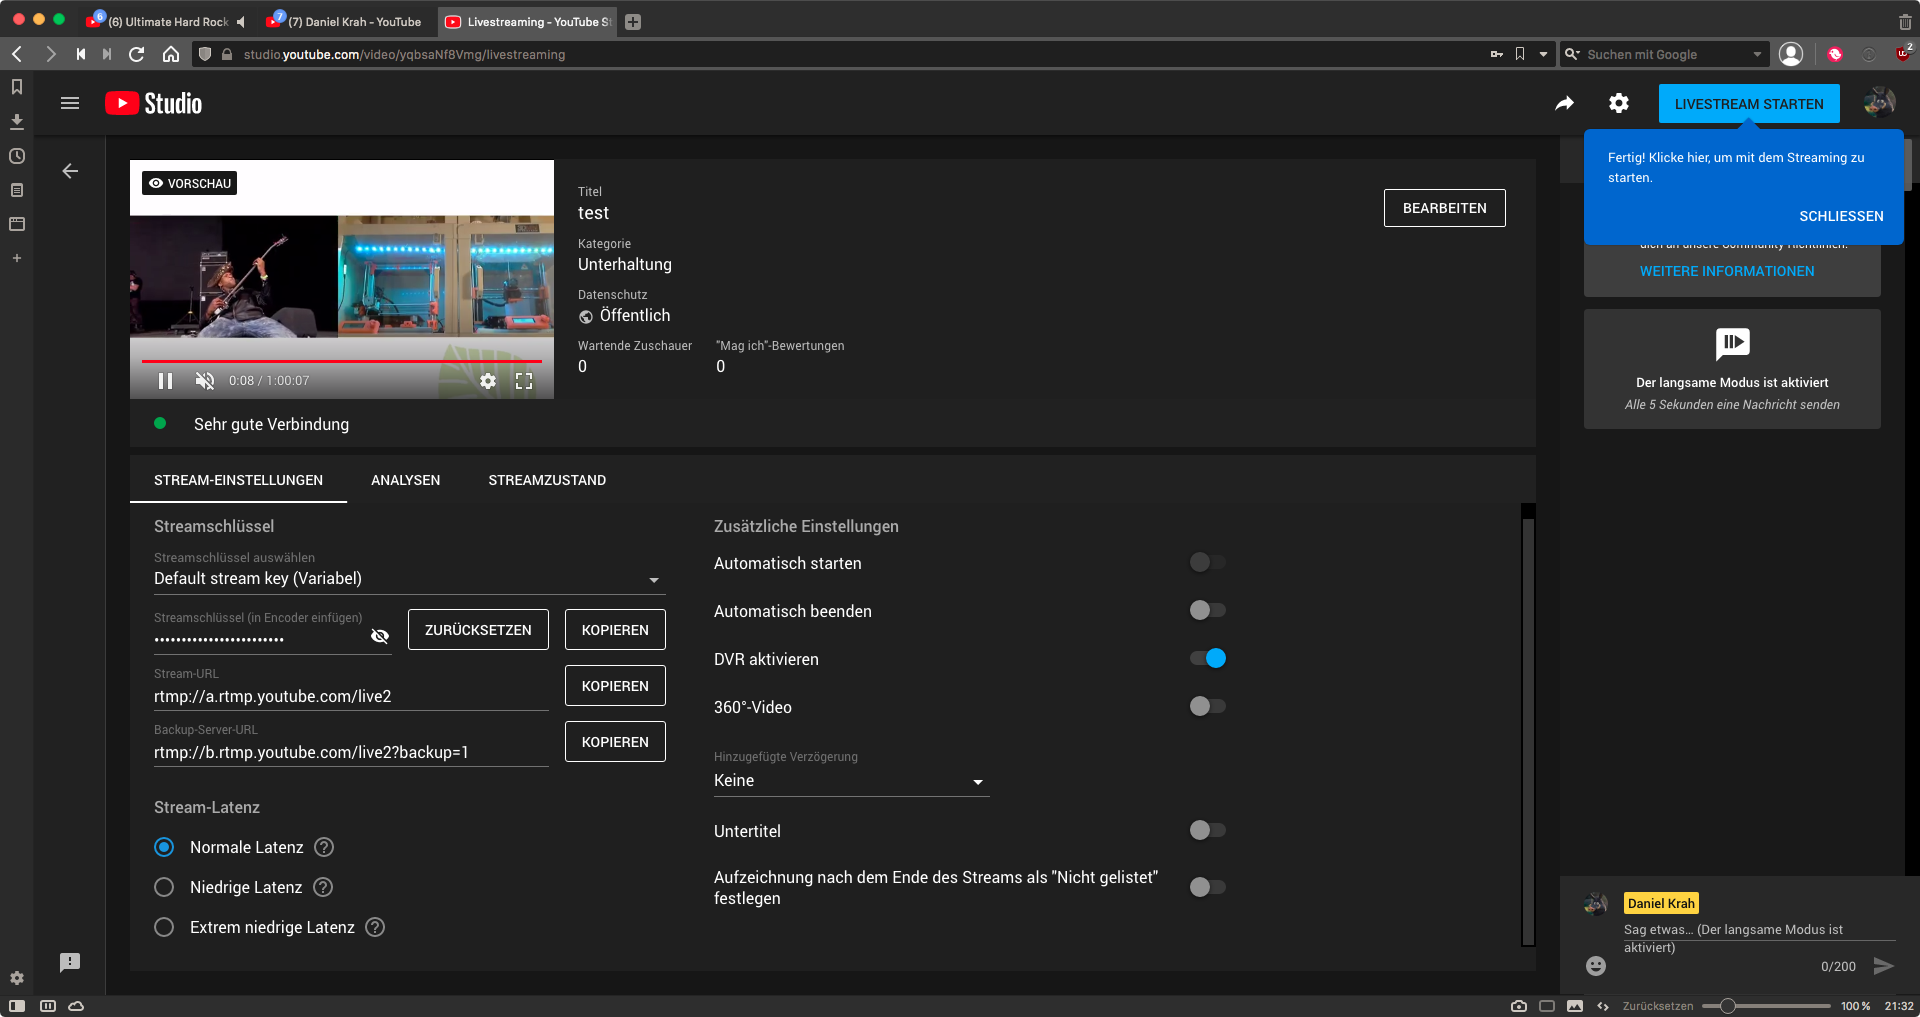
\includegraphics[width=0.7\textwidth]{./pictures/OBSYOutubeConnected.png}
\end{center}



% {\vspace{-0.6cm}}
\begin{center}
  \textbf{Während der Stream started sieht man einen rotierenden Kreis in der Vorschau.} \\
  {\vspace{0.3cm}}
  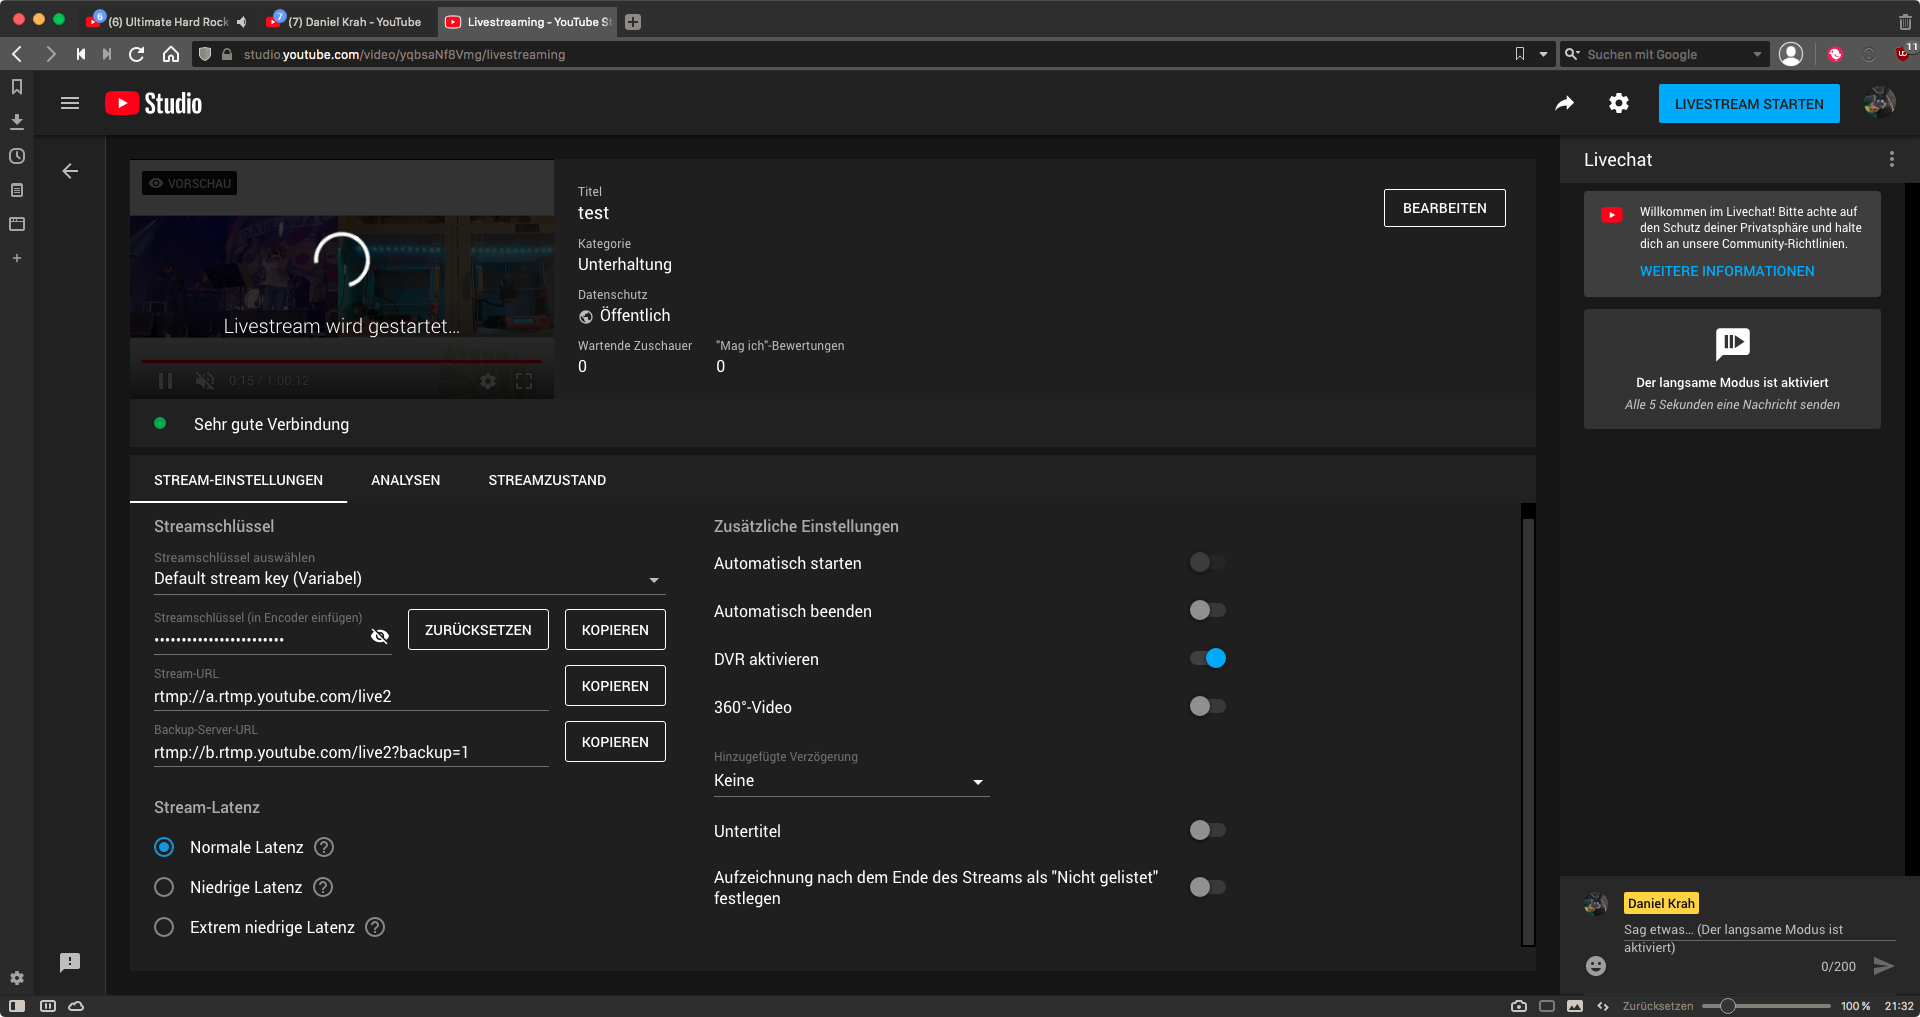
\includegraphics[width=0.7\textwidth]{./pictures/OBSYOutubeConnected-START.png}
\end{center}

\newpage
% {\vspace{-0.6cm}}
\begin{center}
  \textbf{Einen Live-Stream kann man auch über Streamlabs OBS starten.} \\
  {\vspace{0.3cm}}
  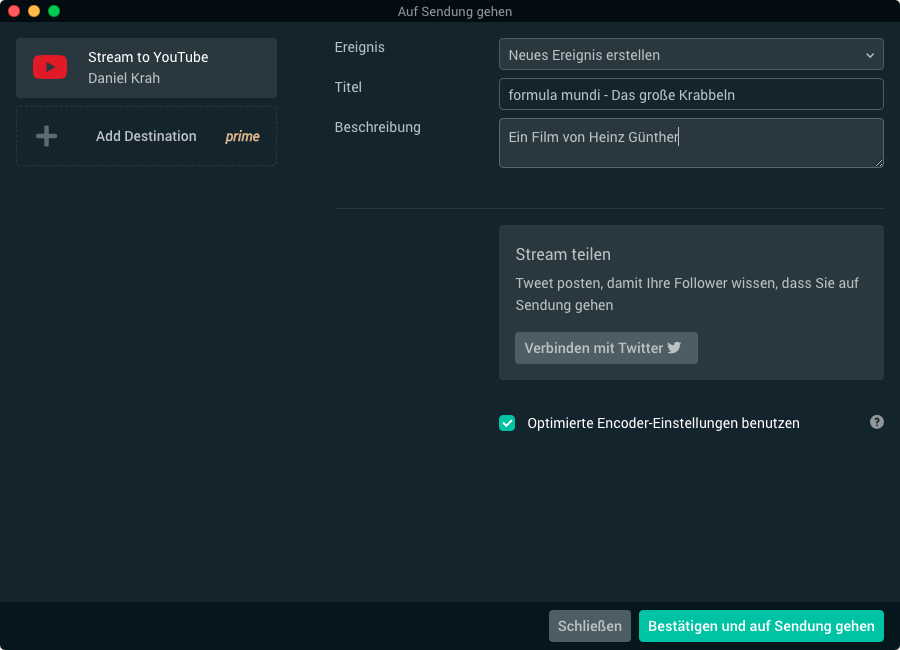
\includegraphics[width=0.9\textwidth]{./pictures/OBSSTUDIO_schnell_aufSendung.png}
\end{center}

% {\vspace{-0.6cm}}
\begin{center}
  \textbf{Vor dem starten des Streams dauert es auch hier etwas.} \\
  {\vspace{0.3cm}}
  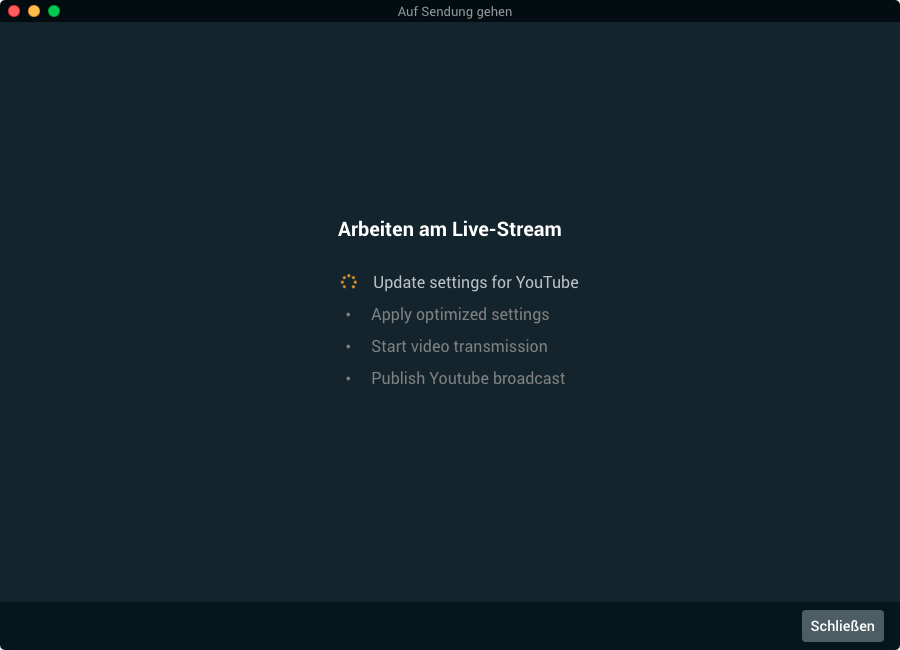
\includegraphics[width=0.7\textwidth]{./pictures/obsStudioIsStartingStream.png}
\end{center}

\newpage
% {\vspace{-0.6cm}}
\begin{center}
  \textbf{Streamlabs OBS hat den Vorteil das es Zugriff auf den Chat hat und man muss nicht den Webbrowser benutzen.} \\
  {\vspace{0.3cm}}
  \includegraphics[width=0.9\textwidth]{./pictures/OBS-STream_Läuft-OBS.png}
\end{center}

% {\vspace{-0.6cm}}
\begin{center}
  \textbf{Hier parallel die Ansicht vom Webbrowser. } \\
  {\vspace{0.3cm}}
  \includegraphics[width=0.9\textwidth]{./pictures/OBS-STream_Läuft-browser.png}
\end{center}



\newpage
% {\vspace{-0.6cm}}
\begin{center}
  \textbf{Natürlich sollte man in den Stream-Einstellungen den Chat konfigurieren} \\
  \textbf{Wichtig sind hierbei die Community-Einstellungen auf welche ich im folgenden Kapitel Youtube Premiere eingehe.} \\
  {\vspace{0.3cm}}
  \includegraphics[width=0.9\textwidth]{./pictures/StreamOptionenLivechat.png}
\end{center}


\sect{Youtube Premiere}

Eine Youtube Premiere kann man einfach über die Webseite starten.
OBS oder OBS Studio werden hier nicht benötigt. \\


\newpage

\sub{Upload des Videos}

{\vspace{0.2cm}}
\begin{center}
  \textbf{Hierfür klickt hierfür auf \quote{Erstellen} rechts oben.} \\
  {\vspace{0.3cm}}
  \includegraphics[width=\textwidth]{./pictures/premiere1.png}
\end{center}



% {\vspace{-0.6cm}}
\begin{center}
  \textbf{Hier ist es wichtig die Zielgruppeneinstellung zu setzen.} \\
  {\vspace{0.3cm}}
  \includegraphics[width=\textwidth]{./pictures/premiere2.png}
\end{center}

\newpage
% {\vspace{-0.6cm}}
\begin{center}
  \textbf{Im nächsten Schritt kann man Infokarten oder einen extra Abspann hinzufügen.} \\
  {\vspace{0.3cm}}
  \includegraphics[width=\textwidth]{./pictures/premiere3.png}
\end{center}


% {\vspace{-0.6cm}}
\begin{center}
  \textbf{Zu guter Letzt legt man das Veröffentlichungsdatum und Uhrzeit fest. } \\
  \textbf{Wichtig ist hierbei das Häkchen bei Premiere zu setzen} \\
  {\vspace{0.3cm}}
  \includegraphics[width=\textwidth]{./pictures/premiere4.png}
\end{center}

\newpage
% {\vspace{-0.6cm}}
\begin{center}
  \textbf{Wenn alles erledigt ist bekommt man noch mal eine Übersicht, sowie vorbereitete Links für Social Media oder die eigene Webseite zum Einbinden.} \\
  {\vspace{0.3cm}}
  \includegraphics[width=\textwidth]{./pictures/premiere5.png}
\end{center}

% {\vspace{-0.6cm}}
\begin{center}
  \textbf{Hier als Beispiel der Quelltext zum einbinden in die Eigene Webseite.} \\
  {\vspace{0.3cm}}
  \includegraphics[width=\textwidth]{./pictures/premiere6.png}
\end{center}

\newpage
\sub{Erweiterte Einstellungen}
% {\vspace{-2.6cm}}
\begin{center}
  \textbf{Als nächstes kann man weitere Einstellungen über das Youtube Studio vornehmen} \\
  \textbf{Die Premiere befindet sich dann unter dem Livestreams-Tab} \\
  {\vspace{0.3cm}}
  \includegraphics[width=\textwidth]{./pictures/premiere7.png}
\end{center}

% {\vspace{-0.6cm}}
\begin{center}
  \textbf{Unter \quote{Weitere Optionen sind die unten abgebildeten Einstellungen zu setzen.}} \\
  \textbf{Zusätzlich kann man den Livechat nach der Premiere ungelöscht lassen.}
  % {\vspace{0.3cm}}
  \includegraphics[width=0.8\textwidth]{./pictures/premiere8.png}
\end{center}

\newpage
\sub{Community Einstellungen}
% {\vspace{-0.6cm}}
\begin{center}
  \textbf{Wenn man auf Community-Einstellungen geklickt hat kann man nun die Schimpfwort-Filter anstellen} \\
  {\vspace{0.3cm}}
  \includegraphics[width=\textwidth]{./pictures/premiere10.png}
\end{center}

% {\vspace{-0.6cm}}
\begin{center}
  \textbf{Im Tab \quote{Automatische Filter} kann man Moderatoren hinzufügen} \\
  {\vspace{0.3cm}}
  \includegraphics[width=\textwidth]{./pictures/premiere9.png}
\end{center}
\newpage


% {\vspace{-0.6cm}}
\begin{center}
  \textbf{Sowie Bestimmte selbst gewählte Wörter Sperren} \\
  {\vspace{0.3cm}}
  \includegraphics[width=\textwidth]{./pictures/premiere11.png}
  \textbf{Das verbieten von Links ist Sinnvoll. Moderatoren können trotzdem Links im Chat posten} \\
\end{center}


Die Premiere verhält sich genau wie ein Livestream. Für den Chat kann man dann einfach den Webbrowser benutzen und benötigt kein Streamlabs OBS/OBS.

\sect{Fazit}

Die Premiere inklusive der Einbindung auf die eigene Webseite ist die beste Möglichkeit das Festival umzusetzen. \\
Durch die likes/dislikes bekommt man auch einen guten Überblick wie gut der jeweilige Film ankam.


% % \end{center}

% sdasasasas \\
% \begin{adjustwidth}{-1cm}{-1cm}% adjust the L and R margins by 1 inch
%   test
% \end{adjustwidth}


% & Streaming unterwegs & Einfache Webcam-Streams & Reproduzierbare Livestreams, die eine einmalige Einrichtung erfordern & Livestream-Einrichtung mit vielen Anpassungsmöglichkeiten \\ \hline
%
% & Schnell und einfach & Schnell und einfach & Produziert & Tent-Poling-Video \\ \hline
% & Gering & Gering & Mittel/Hoch & Hoch \\ \hline
% & Mobiltelefon mit Kamera & Computer mit Webcam & Computer mit Webcam und Streamingsoftware & Computer Kamera Streamingsoftware \\ \hline
%   & Livestream in wenigen Schritten über ein Handy starteb & Livestream mit wenigen Klicks starten & Eine Liveadresse für wiederholbare Livestreams & Eine benutzerdefinierte Live-veranstaltung erstellen, welche auch ein Multicamstream sein kann. \\ \hline



% \newlength{\breite}
% \breite25mm
% \begin{tabular}{|p{\breite}|p{\breite}|p{\breite}|p{\breite}|}
% \hline
% \multicolumn{2}{|l|}{Feld über zwei Spalten}feld&Feld&Feld\\
% \hline
% Feld&Feld&\multicolumn{2}{|l|}{Feld über zwei Spalten}\\
% \hline
% %Feld&\multirow{2}{3cm}{Feld über zwei Zeilen}&Feld\\
% Feld&\multirow{2}{\breite}{Feld über zwei Zeilen}&\multicolumn{2}{|p{3cm}|}{\multirow{2}{5cm}{Feld über zwei Zeilen und zwei Spalten}}\\
% \cline{0-0}
% Feld&&\multicolumn{2}{|c|}{}\\
% \hline
% \end{tabular}

% \begin{table}[htb]
%       \begin{tabular*}{\linewidth}{@{\extracolsep{\fill}}*8l@{}} \toprule
%       Spalte1 & Spalte2 & Spalte3 & Spalte4 & Spalte5 & Spalte6 & Spalte7 & Spalte8 \\ \midrule
%       AA      & BB      & CC      & DD      & EE      & FF      & GG      & HH      \\
%       AA      & BB      & CC      & DD      & EE      & FF      & GG      & HH      \\ \bottomrule
%     \end{tabular*}
% \end{table}

\sect{Vorbereitung des Streams}

Bei einem Livestream gibt es einiges bezüglich des Chats zu beachten:
\begin{itemize}
  \item Moderatoren sollten vor einem Chat zugewiesen sein.
  \item Blockieren von unangemessenen Wörtern oder Links aktivieren.
  \item Langsamen Modus aktivieren damit Zuschauer nicht den Chat zuspammen können.
  \item \grqq{}Zur Überprüfung zurückhalten\grqq{} aktivieren damit problematische Wörter nicht im chat erscheinen.
\end{itemize}

\sect{Geplante Veröffentlichungen}


\sect{Während des Streams}
\sect{Voting}
\sect{Fazit}


% \includegraphics[scale=0.5]{./pictures/vordemstream.png}
%
% \includegraphics[scale=0.5]{./pictures/livechat.png}

% \includegraphics[scale=0.5]{./pictures/preflightchecks.png}
% \includegraphics[scale=0.5]{./pictures/streamingarten.png}
%
%
%















%
% \begin{tabular}{ll}
% \centering
% \glqq Text\grqq{} und \flqq Text\frqq  & \verb+ \glqq Text\grqq{} und \flqq Text\frqq+\\
% \glq Text\grq{} und \flq Text\frq  & \verb+ \glq Text\grq{} und \flq Text\frq+
% \end{tabular}





% \definecolor{fulda_green}{rgb}{.38,.74,.10}
% \definecolor{fulda_lightgreen}{rgb}{.64,.85,.40}
% \definecolor{fulda_lightgray}{gray}{.4}
% \definecolor{fulda_subtitle}{rgb}{.38,.74,.10}
% \definecolor{fulda_title}{gray}{.0}
% \definecolor{fulda_chapter}{rgb}{.38,.74,.10}
% \definecolor{fulda_section}{rgb}{.38,.74,.10}
% \definecolor{fulda_subsection}{gray}{.4}
% \definecolor{fulda_part}{gray}{1}
% \definecolor{fulda_partnumber}{rgb}{.79,1,.55}
% \definecolor{fulda_partback}{rgb}{.64,.85,.40}
% \definecolor{fulda_highlighttitle}{rgb}{.38,.74,.10}
% \definecolor{fulda_highlightbody}{rgb}{.79,1,.55}
% \definecolor{fulda_highlighttitletext}{gray}{1}
% \definecolor{lightgray}{rgb}{0.93,0.95,1.0}
% \definecolor{darkgreen}{RGB}{82,130,179}


% \input{strukturen.tex}
% \input{threadsProzesse.tex}

%=========================================================================================================================
%
%-------------END
\end{document}
